
    




    
\documentclass[11pt]{article}

    
    \usepackage[breakable]{tcolorbox}
    \tcbset{nobeforeafter} % prevents tcolorboxes being placing in paragraphs
    \usepackage{float}
    \floatplacement{figure}{H} % forces figures to be placed at the correct location
    
    \usepackage[T1]{fontenc}
    % Nicer default font (+ math font) than Computer Modern for most use cases
    \usepackage{mathpazo}

    % Basic figure setup, for now with no caption control since it's done
    % automatically by Pandoc (which extracts ![](path) syntax from Markdown).
    \usepackage{graphicx}
    % We will generate all images so they have a width \maxwidth. This means
    % that they will get their normal width if they fit onto the page, but
    % are scaled down if they would overflow the margins.
    \makeatletter
    \def\maxwidth{\ifdim\Gin@nat@width>\linewidth\linewidth
    \else\Gin@nat@width\fi}
    \makeatother
    \let\Oldincludegraphics\includegraphics
    % Set max figure width to be 80% of text width, for now hardcoded.
    \renewcommand{\includegraphics}[1]{\Oldincludegraphics[width=.8\maxwidth]{#1}}
    % Ensure that by default, figures have no caption (until we provide a
    % proper Figure object with a Caption API and a way to capture that
    % in the conversion process - todo).
    \usepackage{caption}
    \DeclareCaptionLabelFormat{nolabel}{}
    \captionsetup{labelformat=nolabel}

    \usepackage{adjustbox} % Used to constrain images to a maximum size 
    \usepackage{xcolor} % Allow colors to be defined
    \usepackage{enumerate} % Needed for markdown enumerations to work
    \usepackage{geometry} % Used to adjust the document margins
    \usepackage{amsmath} % Equations
    \usepackage{amssymb} % Equations
    \usepackage{textcomp} % defines textquotesingle
    % Hack from http://tex.stackexchange.com/a/47451/13684:
    \AtBeginDocument{%
        \def\PYZsq{\textquotesingle}% Upright quotes in Pygmentized code
    }
    \usepackage{upquote} % Upright quotes for verbatim code
    \usepackage{eurosym} % defines \euro
    \usepackage[mathletters]{ucs} % Extended unicode (utf-8) support
    \usepackage[utf8x]{inputenc} % Allow utf-8 characters in the tex document
    \usepackage{fancyvrb} % verbatim replacement that allows latex
    \usepackage{grffile} % extends the file name processing of package graphics 
                         % to support a larger range 
    % The hyperref package gives us a pdf with properly built
    % internal navigation ('pdf bookmarks' for the table of contents,
    % internal cross-reference links, web links for URLs, etc.)
    \usepackage{hyperref}
    \usepackage{longtable} % longtable support required by pandoc >1.10
    \usepackage{booktabs}  % table support for pandoc > 1.12.2
    \usepackage[inline]{enumitem} % IRkernel/repr support (it uses the enumerate* environment)
    \usepackage[normalem]{ulem} % ulem is needed to support strikethroughs (\sout)
                                % normalem makes italics be italics, not underlines
    \usepackage{mathrsfs}
    

    
    % Colors for the hyperref package
    \definecolor{urlcolor}{rgb}{0,.145,.698}
    \definecolor{linkcolor}{rgb}{.71,0.21,0.01}
    \definecolor{citecolor}{rgb}{.12,.54,.11}

    % ANSI colors
    \definecolor{ansi-black}{HTML}{3E424D}
    \definecolor{ansi-black-intense}{HTML}{282C36}
    \definecolor{ansi-red}{HTML}{E75C58}
    \definecolor{ansi-red-intense}{HTML}{B22B31}
    \definecolor{ansi-green}{HTML}{00A250}
    \definecolor{ansi-green-intense}{HTML}{007427}
    \definecolor{ansi-yellow}{HTML}{DDB62B}
    \definecolor{ansi-yellow-intense}{HTML}{B27D12}
    \definecolor{ansi-blue}{HTML}{208FFB}
    \definecolor{ansi-blue-intense}{HTML}{0065CA}
    \definecolor{ansi-magenta}{HTML}{D160C4}
    \definecolor{ansi-magenta-intense}{HTML}{A03196}
    \definecolor{ansi-cyan}{HTML}{60C6C8}
    \definecolor{ansi-cyan-intense}{HTML}{258F8F}
    \definecolor{ansi-white}{HTML}{C5C1B4}
    \definecolor{ansi-white-intense}{HTML}{A1A6B2}
    \definecolor{ansi-default-inverse-fg}{HTML}{FFFFFF}
    \definecolor{ansi-default-inverse-bg}{HTML}{000000}

    % commands and environments needed by pandoc snippets
    % extracted from the output of `pandoc -s`
    \providecommand{\tightlist}{%
      \setlength{\itemsep}{0pt}\setlength{\parskip}{0pt}}
    \DefineVerbatimEnvironment{Highlighting}{Verbatim}{commandchars=\\\{\}}
    % Add ',fontsize=\small' for more characters per line
    \newenvironment{Shaded}{}{}
    \newcommand{\KeywordTok}[1]{\textcolor[rgb]{0.00,0.44,0.13}{\textbf{{#1}}}}
    \newcommand{\DataTypeTok}[1]{\textcolor[rgb]{0.56,0.13,0.00}{{#1}}}
    \newcommand{\DecValTok}[1]{\textcolor[rgb]{0.25,0.63,0.44}{{#1}}}
    \newcommand{\BaseNTok}[1]{\textcolor[rgb]{0.25,0.63,0.44}{{#1}}}
    \newcommand{\FloatTok}[1]{\textcolor[rgb]{0.25,0.63,0.44}{{#1}}}
    \newcommand{\CharTok}[1]{\textcolor[rgb]{0.25,0.44,0.63}{{#1}}}
    \newcommand{\StringTok}[1]{\textcolor[rgb]{0.25,0.44,0.63}{{#1}}}
    \newcommand{\CommentTok}[1]{\textcolor[rgb]{0.38,0.63,0.69}{\textit{{#1}}}}
    \newcommand{\OtherTok}[1]{\textcolor[rgb]{0.00,0.44,0.13}{{#1}}}
    \newcommand{\AlertTok}[1]{\textcolor[rgb]{1.00,0.00,0.00}{\textbf{{#1}}}}
    \newcommand{\FunctionTok}[1]{\textcolor[rgb]{0.02,0.16,0.49}{{#1}}}
    \newcommand{\RegionMarkerTok}[1]{{#1}}
    \newcommand{\ErrorTok}[1]{\textcolor[rgb]{1.00,0.00,0.00}{\textbf{{#1}}}}
    \newcommand{\NormalTok}[1]{{#1}}
    
    % Additional commands for more recent versions of Pandoc
    \newcommand{\ConstantTok}[1]{\textcolor[rgb]{0.53,0.00,0.00}{{#1}}}
    \newcommand{\SpecialCharTok}[1]{\textcolor[rgb]{0.25,0.44,0.63}{{#1}}}
    \newcommand{\VerbatimStringTok}[1]{\textcolor[rgb]{0.25,0.44,0.63}{{#1}}}
    \newcommand{\SpecialStringTok}[1]{\textcolor[rgb]{0.73,0.40,0.53}{{#1}}}
    \newcommand{\ImportTok}[1]{{#1}}
    \newcommand{\DocumentationTok}[1]{\textcolor[rgb]{0.73,0.13,0.13}{\textit{{#1}}}}
    \newcommand{\AnnotationTok}[1]{\textcolor[rgb]{0.38,0.63,0.69}{\textbf{\textit{{#1}}}}}
    \newcommand{\CommentVarTok}[1]{\textcolor[rgb]{0.38,0.63,0.69}{\textbf{\textit{{#1}}}}}
    \newcommand{\VariableTok}[1]{\textcolor[rgb]{0.10,0.09,0.49}{{#1}}}
    \newcommand{\ControlFlowTok}[1]{\textcolor[rgb]{0.00,0.44,0.13}{\textbf{{#1}}}}
    \newcommand{\OperatorTok}[1]{\textcolor[rgb]{0.40,0.40,0.40}{{#1}}}
    \newcommand{\BuiltInTok}[1]{{#1}}
    \newcommand{\ExtensionTok}[1]{{#1}}
    \newcommand{\PreprocessorTok}[1]{\textcolor[rgb]{0.74,0.48,0.00}{{#1}}}
    \newcommand{\AttributeTok}[1]{\textcolor[rgb]{0.49,0.56,0.16}{{#1}}}
    \newcommand{\InformationTok}[1]{\textcolor[rgb]{0.38,0.63,0.69}{\textbf{\textit{{#1}}}}}
    \newcommand{\WarningTok}[1]{\textcolor[rgb]{0.38,0.63,0.69}{\textbf{\textit{{#1}}}}}
    
    
    % Define a nice break command that doesn't care if a line doesn't already
    % exist.
    \def\br{\hspace*{\fill} \\* }
    % Math Jax compatibility definitions
    \def\gt{>}
    \def\lt{<}
    \let\Oldtex\TeX
    \let\Oldlatex\LaTeX
    \renewcommand{\TeX}{\textrm{\Oldtex}}
    \renewcommand{\LaTeX}{\textrm{\Oldlatex}}
    % Document parameters
    % Document title
    \title{Lab2}
    
    
    
    
    
% Pygments definitions
\makeatletter
\def\PY@reset{\let\PY@it=\relax \let\PY@bf=\relax%
    \let\PY@ul=\relax \let\PY@tc=\relax%
    \let\PY@bc=\relax \let\PY@ff=\relax}
\def\PY@tok#1{\csname PY@tok@#1\endcsname}
\def\PY@toks#1+{\ifx\relax#1\empty\else%
    \PY@tok{#1}\expandafter\PY@toks\fi}
\def\PY@do#1{\PY@bc{\PY@tc{\PY@ul{%
    \PY@it{\PY@bf{\PY@ff{#1}}}}}}}
\def\PY#1#2{\PY@reset\PY@toks#1+\relax+\PY@do{#2}}

\expandafter\def\csname PY@tok@w\endcsname{\def\PY@tc##1{\textcolor[rgb]{0.73,0.73,0.73}{##1}}}
\expandafter\def\csname PY@tok@c\endcsname{\let\PY@it=\textit\def\PY@tc##1{\textcolor[rgb]{0.25,0.50,0.50}{##1}}}
\expandafter\def\csname PY@tok@cp\endcsname{\def\PY@tc##1{\textcolor[rgb]{0.74,0.48,0.00}{##1}}}
\expandafter\def\csname PY@tok@k\endcsname{\let\PY@bf=\textbf\def\PY@tc##1{\textcolor[rgb]{0.00,0.50,0.00}{##1}}}
\expandafter\def\csname PY@tok@kp\endcsname{\def\PY@tc##1{\textcolor[rgb]{0.00,0.50,0.00}{##1}}}
\expandafter\def\csname PY@tok@kt\endcsname{\def\PY@tc##1{\textcolor[rgb]{0.69,0.00,0.25}{##1}}}
\expandafter\def\csname PY@tok@o\endcsname{\def\PY@tc##1{\textcolor[rgb]{0.40,0.40,0.40}{##1}}}
\expandafter\def\csname PY@tok@ow\endcsname{\let\PY@bf=\textbf\def\PY@tc##1{\textcolor[rgb]{0.67,0.13,1.00}{##1}}}
\expandafter\def\csname PY@tok@nb\endcsname{\def\PY@tc##1{\textcolor[rgb]{0.00,0.50,0.00}{##1}}}
\expandafter\def\csname PY@tok@nf\endcsname{\def\PY@tc##1{\textcolor[rgb]{0.00,0.00,1.00}{##1}}}
\expandafter\def\csname PY@tok@nc\endcsname{\let\PY@bf=\textbf\def\PY@tc##1{\textcolor[rgb]{0.00,0.00,1.00}{##1}}}
\expandafter\def\csname PY@tok@nn\endcsname{\let\PY@bf=\textbf\def\PY@tc##1{\textcolor[rgb]{0.00,0.00,1.00}{##1}}}
\expandafter\def\csname PY@tok@ne\endcsname{\let\PY@bf=\textbf\def\PY@tc##1{\textcolor[rgb]{0.82,0.25,0.23}{##1}}}
\expandafter\def\csname PY@tok@nv\endcsname{\def\PY@tc##1{\textcolor[rgb]{0.10,0.09,0.49}{##1}}}
\expandafter\def\csname PY@tok@no\endcsname{\def\PY@tc##1{\textcolor[rgb]{0.53,0.00,0.00}{##1}}}
\expandafter\def\csname PY@tok@nl\endcsname{\def\PY@tc##1{\textcolor[rgb]{0.63,0.63,0.00}{##1}}}
\expandafter\def\csname PY@tok@ni\endcsname{\let\PY@bf=\textbf\def\PY@tc##1{\textcolor[rgb]{0.60,0.60,0.60}{##1}}}
\expandafter\def\csname PY@tok@na\endcsname{\def\PY@tc##1{\textcolor[rgb]{0.49,0.56,0.16}{##1}}}
\expandafter\def\csname PY@tok@nt\endcsname{\let\PY@bf=\textbf\def\PY@tc##1{\textcolor[rgb]{0.00,0.50,0.00}{##1}}}
\expandafter\def\csname PY@tok@nd\endcsname{\def\PY@tc##1{\textcolor[rgb]{0.67,0.13,1.00}{##1}}}
\expandafter\def\csname PY@tok@s\endcsname{\def\PY@tc##1{\textcolor[rgb]{0.73,0.13,0.13}{##1}}}
\expandafter\def\csname PY@tok@sd\endcsname{\let\PY@it=\textit\def\PY@tc##1{\textcolor[rgb]{0.73,0.13,0.13}{##1}}}
\expandafter\def\csname PY@tok@si\endcsname{\let\PY@bf=\textbf\def\PY@tc##1{\textcolor[rgb]{0.73,0.40,0.53}{##1}}}
\expandafter\def\csname PY@tok@se\endcsname{\let\PY@bf=\textbf\def\PY@tc##1{\textcolor[rgb]{0.73,0.40,0.13}{##1}}}
\expandafter\def\csname PY@tok@sr\endcsname{\def\PY@tc##1{\textcolor[rgb]{0.73,0.40,0.53}{##1}}}
\expandafter\def\csname PY@tok@ss\endcsname{\def\PY@tc##1{\textcolor[rgb]{0.10,0.09,0.49}{##1}}}
\expandafter\def\csname PY@tok@sx\endcsname{\def\PY@tc##1{\textcolor[rgb]{0.00,0.50,0.00}{##1}}}
\expandafter\def\csname PY@tok@m\endcsname{\def\PY@tc##1{\textcolor[rgb]{0.40,0.40,0.40}{##1}}}
\expandafter\def\csname PY@tok@gh\endcsname{\let\PY@bf=\textbf\def\PY@tc##1{\textcolor[rgb]{0.00,0.00,0.50}{##1}}}
\expandafter\def\csname PY@tok@gu\endcsname{\let\PY@bf=\textbf\def\PY@tc##1{\textcolor[rgb]{0.50,0.00,0.50}{##1}}}
\expandafter\def\csname PY@tok@gd\endcsname{\def\PY@tc##1{\textcolor[rgb]{0.63,0.00,0.00}{##1}}}
\expandafter\def\csname PY@tok@gi\endcsname{\def\PY@tc##1{\textcolor[rgb]{0.00,0.63,0.00}{##1}}}
\expandafter\def\csname PY@tok@gr\endcsname{\def\PY@tc##1{\textcolor[rgb]{1.00,0.00,0.00}{##1}}}
\expandafter\def\csname PY@tok@ge\endcsname{\let\PY@it=\textit}
\expandafter\def\csname PY@tok@gs\endcsname{\let\PY@bf=\textbf}
\expandafter\def\csname PY@tok@gp\endcsname{\let\PY@bf=\textbf\def\PY@tc##1{\textcolor[rgb]{0.00,0.00,0.50}{##1}}}
\expandafter\def\csname PY@tok@go\endcsname{\def\PY@tc##1{\textcolor[rgb]{0.53,0.53,0.53}{##1}}}
\expandafter\def\csname PY@tok@gt\endcsname{\def\PY@tc##1{\textcolor[rgb]{0.00,0.27,0.87}{##1}}}
\expandafter\def\csname PY@tok@err\endcsname{\def\PY@bc##1{\setlength{\fboxsep}{0pt}\fcolorbox[rgb]{1.00,0.00,0.00}{1,1,1}{\strut ##1}}}
\expandafter\def\csname PY@tok@kc\endcsname{\let\PY@bf=\textbf\def\PY@tc##1{\textcolor[rgb]{0.00,0.50,0.00}{##1}}}
\expandafter\def\csname PY@tok@kd\endcsname{\let\PY@bf=\textbf\def\PY@tc##1{\textcolor[rgb]{0.00,0.50,0.00}{##1}}}
\expandafter\def\csname PY@tok@kn\endcsname{\let\PY@bf=\textbf\def\PY@tc##1{\textcolor[rgb]{0.00,0.50,0.00}{##1}}}
\expandafter\def\csname PY@tok@kr\endcsname{\let\PY@bf=\textbf\def\PY@tc##1{\textcolor[rgb]{0.00,0.50,0.00}{##1}}}
\expandafter\def\csname PY@tok@bp\endcsname{\def\PY@tc##1{\textcolor[rgb]{0.00,0.50,0.00}{##1}}}
\expandafter\def\csname PY@tok@fm\endcsname{\def\PY@tc##1{\textcolor[rgb]{0.00,0.00,1.00}{##1}}}
\expandafter\def\csname PY@tok@vc\endcsname{\def\PY@tc##1{\textcolor[rgb]{0.10,0.09,0.49}{##1}}}
\expandafter\def\csname PY@tok@vg\endcsname{\def\PY@tc##1{\textcolor[rgb]{0.10,0.09,0.49}{##1}}}
\expandafter\def\csname PY@tok@vi\endcsname{\def\PY@tc##1{\textcolor[rgb]{0.10,0.09,0.49}{##1}}}
\expandafter\def\csname PY@tok@vm\endcsname{\def\PY@tc##1{\textcolor[rgb]{0.10,0.09,0.49}{##1}}}
\expandafter\def\csname PY@tok@sa\endcsname{\def\PY@tc##1{\textcolor[rgb]{0.73,0.13,0.13}{##1}}}
\expandafter\def\csname PY@tok@sb\endcsname{\def\PY@tc##1{\textcolor[rgb]{0.73,0.13,0.13}{##1}}}
\expandafter\def\csname PY@tok@sc\endcsname{\def\PY@tc##1{\textcolor[rgb]{0.73,0.13,0.13}{##1}}}
\expandafter\def\csname PY@tok@dl\endcsname{\def\PY@tc##1{\textcolor[rgb]{0.73,0.13,0.13}{##1}}}
\expandafter\def\csname PY@tok@s2\endcsname{\def\PY@tc##1{\textcolor[rgb]{0.73,0.13,0.13}{##1}}}
\expandafter\def\csname PY@tok@sh\endcsname{\def\PY@tc##1{\textcolor[rgb]{0.73,0.13,0.13}{##1}}}
\expandafter\def\csname PY@tok@s1\endcsname{\def\PY@tc##1{\textcolor[rgb]{0.73,0.13,0.13}{##1}}}
\expandafter\def\csname PY@tok@mb\endcsname{\def\PY@tc##1{\textcolor[rgb]{0.40,0.40,0.40}{##1}}}
\expandafter\def\csname PY@tok@mf\endcsname{\def\PY@tc##1{\textcolor[rgb]{0.40,0.40,0.40}{##1}}}
\expandafter\def\csname PY@tok@mh\endcsname{\def\PY@tc##1{\textcolor[rgb]{0.40,0.40,0.40}{##1}}}
\expandafter\def\csname PY@tok@mi\endcsname{\def\PY@tc##1{\textcolor[rgb]{0.40,0.40,0.40}{##1}}}
\expandafter\def\csname PY@tok@il\endcsname{\def\PY@tc##1{\textcolor[rgb]{0.40,0.40,0.40}{##1}}}
\expandafter\def\csname PY@tok@mo\endcsname{\def\PY@tc##1{\textcolor[rgb]{0.40,0.40,0.40}{##1}}}
\expandafter\def\csname PY@tok@ch\endcsname{\let\PY@it=\textit\def\PY@tc##1{\textcolor[rgb]{0.25,0.50,0.50}{##1}}}
\expandafter\def\csname PY@tok@cm\endcsname{\let\PY@it=\textit\def\PY@tc##1{\textcolor[rgb]{0.25,0.50,0.50}{##1}}}
\expandafter\def\csname PY@tok@cpf\endcsname{\let\PY@it=\textit\def\PY@tc##1{\textcolor[rgb]{0.25,0.50,0.50}{##1}}}
\expandafter\def\csname PY@tok@c1\endcsname{\let\PY@it=\textit\def\PY@tc##1{\textcolor[rgb]{0.25,0.50,0.50}{##1}}}
\expandafter\def\csname PY@tok@cs\endcsname{\let\PY@it=\textit\def\PY@tc##1{\textcolor[rgb]{0.25,0.50,0.50}{##1}}}

\def\PYZbs{\char`\\}
\def\PYZus{\char`\_}
\def\PYZob{\char`\{}
\def\PYZcb{\char`\}}
\def\PYZca{\char`\^}
\def\PYZam{\char`\&}
\def\PYZlt{\char`\<}
\def\PYZgt{\char`\>}
\def\PYZsh{\char`\#}
\def\PYZpc{\char`\%}
\def\PYZdl{\char`\$}
\def\PYZhy{\char`\-}
\def\PYZsq{\char`\'}
\def\PYZdq{\char`\"}
\def\PYZti{\char`\~}
% for compatibility with earlier versions
\def\PYZat{@}
\def\PYZlb{[}
\def\PYZrb{]}
\makeatother


    % For linebreaks inside Verbatim environment from package fancyvrb. 
    \makeatletter
        \newbox\Wrappedcontinuationbox 
        \newbox\Wrappedvisiblespacebox 
        \newcommand*\Wrappedvisiblespace {\textcolor{red}{\textvisiblespace}} 
        \newcommand*\Wrappedcontinuationsymbol {\textcolor{red}{\llap{\tiny$\m@th\hookrightarrow$}}} 
        \newcommand*\Wrappedcontinuationindent {3ex } 
        \newcommand*\Wrappedafterbreak {\kern\Wrappedcontinuationindent\copy\Wrappedcontinuationbox} 
        % Take advantage of the already applied Pygments mark-up to insert 
        % potential linebreaks for TeX processing. 
        %        {, <, #, %, $, ' and ": go to next line. 
        %        _, }, ^, &, >, - and ~: stay at end of broken line. 
        % Use of \textquotesingle for straight quote. 
        \newcommand*\Wrappedbreaksatspecials {% 
            \def\PYGZus{\discretionary{\char`\_}{\Wrappedafterbreak}{\char`\_}}% 
            \def\PYGZob{\discretionary{}{\Wrappedafterbreak\char`\{}{\char`\{}}% 
            \def\PYGZcb{\discretionary{\char`\}}{\Wrappedafterbreak}{\char`\}}}% 
            \def\PYGZca{\discretionary{\char`\^}{\Wrappedafterbreak}{\char`\^}}% 
            \def\PYGZam{\discretionary{\char`\&}{\Wrappedafterbreak}{\char`\&}}% 
            \def\PYGZlt{\discretionary{}{\Wrappedafterbreak\char`\<}{\char`\<}}% 
            \def\PYGZgt{\discretionary{\char`\>}{\Wrappedafterbreak}{\char`\>}}% 
            \def\PYGZsh{\discretionary{}{\Wrappedafterbreak\char`\#}{\char`\#}}% 
            \def\PYGZpc{\discretionary{}{\Wrappedafterbreak\char`\%}{\char`\%}}% 
            \def\PYGZdl{\discretionary{}{\Wrappedafterbreak\char`\$}{\char`\$}}% 
            \def\PYGZhy{\discretionary{\char`\-}{\Wrappedafterbreak}{\char`\-}}% 
            \def\PYGZsq{\discretionary{}{\Wrappedafterbreak\textquotesingle}{\textquotesingle}}% 
            \def\PYGZdq{\discretionary{}{\Wrappedafterbreak\char`\"}{\char`\"}}% 
            \def\PYGZti{\discretionary{\char`\~}{\Wrappedafterbreak}{\char`\~}}% 
        } 
        % Some characters . , ; ? ! / are not pygmentized. 
        % This macro makes them "active" and they will insert potential linebreaks 
        \newcommand*\Wrappedbreaksatpunct {% 
            \lccode`\~`\.\lowercase{\def~}{\discretionary{\hbox{\char`\.}}{\Wrappedafterbreak}{\hbox{\char`\.}}}% 
            \lccode`\~`\,\lowercase{\def~}{\discretionary{\hbox{\char`\,}}{\Wrappedafterbreak}{\hbox{\char`\,}}}% 
            \lccode`\~`\;\lowercase{\def~}{\discretionary{\hbox{\char`\;}}{\Wrappedafterbreak}{\hbox{\char`\;}}}% 
            \lccode`\~`\:\lowercase{\def~}{\discretionary{\hbox{\char`\:}}{\Wrappedafterbreak}{\hbox{\char`\:}}}% 
            \lccode`\~`\?\lowercase{\def~}{\discretionary{\hbox{\char`\?}}{\Wrappedafterbreak}{\hbox{\char`\?}}}% 
            \lccode`\~`\!\lowercase{\def~}{\discretionary{\hbox{\char`\!}}{\Wrappedafterbreak}{\hbox{\char`\!}}}% 
            \lccode`\~`\/\lowercase{\def~}{\discretionary{\hbox{\char`\/}}{\Wrappedafterbreak}{\hbox{\char`\/}}}% 
            \catcode`\.\active
            \catcode`\,\active 
            \catcode`\;\active
            \catcode`\:\active
            \catcode`\?\active
            \catcode`\!\active
            \catcode`\/\active 
            \lccode`\~`\~ 	
        }
    \makeatother

    \let\OriginalVerbatim=\Verbatim
    \makeatletter
    \renewcommand{\Verbatim}[1][1]{%
        %\parskip\z@skip
        \sbox\Wrappedcontinuationbox {\Wrappedcontinuationsymbol}%
        \sbox\Wrappedvisiblespacebox {\FV@SetupFont\Wrappedvisiblespace}%
        \def\FancyVerbFormatLine ##1{\hsize\linewidth
            \vtop{\raggedright\hyphenpenalty\z@\exhyphenpenalty\z@
                \doublehyphendemerits\z@\finalhyphendemerits\z@
                \strut ##1\strut}%
        }%
        % If the linebreak is at a space, the latter will be displayed as visible
        % space at end of first line, and a continuation symbol starts next line.
        % Stretch/shrink are however usually zero for typewriter font.
        \def\FV@Space {%
            \nobreak\hskip\z@ plus\fontdimen3\font minus\fontdimen4\font
            \discretionary{\copy\Wrappedvisiblespacebox}{\Wrappedafterbreak}
            {\kern\fontdimen2\font}%
        }%
        
        % Allow breaks at special characters using \PYG... macros.
        \Wrappedbreaksatspecials
        % Breaks at punctuation characters . , ; ? ! and / need catcode=\active 	
        \OriginalVerbatim[#1,codes*=\Wrappedbreaksatpunct]%
    }
    \makeatother

    % Exact colors from NB
    \definecolor{incolor}{HTML}{303F9F}
    \definecolor{outcolor}{HTML}{D84315}
    \definecolor{cellborder}{HTML}{CFCFCF}
    \definecolor{cellbackground}{HTML}{F7F7F7}
    
    % prompt
    \newcommand{\prompt}[4]{
        \llap{{\color{#2}[#3]: #4}}\vspace{-1.25em}
    }
    

    
    % Prevent overflowing lines due to hard-to-break entities
    \sloppy 
    % Setup hyperref package
    \hypersetup{
      breaklinks=true,  % so long urls are correctly broken across lines
      colorlinks=true,
      urlcolor=urlcolor,
      linkcolor=linkcolor,
      citecolor=citecolor,
      }
    % Slightly bigger margins than the latex defaults
    
    \geometry{verbose,tmargin=1in,bmargin=1in,lmargin=1in,rmargin=1in}
    
    

    \begin{document}
    
    
    \maketitle
    
    

    
    \hypertarget{experiment-1---linear-polarization-and-maluss-law}{%
\subsection{Experiment 1 - Linear Polarization and Malus's
Law}\label{experiment-1---linear-polarization-and-maluss-law}}

\hypertarget{objective}{%
\paragraph{Objective:}\label{objective}}

\begin{itemize}
\tightlist
\item
  Learn to recognize linearly polarized light from unpolarized light
\item
  Test Malus's Law for linearly polarized light
\end{itemize}

\hypertarget{method}{%
\paragraph{Method:}\label{method}}

First objective:

We used the setups shown in the diagrams of part 1.1 in the lab manual.
To sum up this part of the experiment, we essentially used linear
polarizers together with various light sources to determine the
polarization of the light coming from different sources.

Second Objective:

Malus's law takes the form,

\[I = I_o \cos^2(\theta_{rel}) + I_{bg}\]

Therefore to test this law we needed to first determine \(I_{bg}\), and
then take data for \(I\) at a variety of \(\theta_{rel}\).

We first set up materials according to the second diagram in section 1.1
of the lab manual, but we substituted the bench lamp for the laser. To
find \(I_{bg}\), we turned off the laser and simply took a reading of
the photodetector in the unlit room.

To test Malus's Law, we fixed the first linear polarizer to emit
vertically polarized light, and then we used the photodetector to
measure the intensity of light coming from the second polarizer at
different angles of the second polarizer. Here the angle of the second
polarizer corresponds to \(\theta_{rel}\) in Malus's law. In the data
analysis section below, we give our experimentally determined value for
\(I_o\).

    \hypertarget{analysis}{%
\paragraph{Analysis:}\label{analysis}}

I will answer each analysis question in the order they appeared in the
lab manual.

Analysis 1: Based on our observations from the first part of the
experiment, the laser beam is neither unpolarized nor fully polarized,
but it appears to be mostly linearly polarized (The beam never fully
vanishes as we rotate the polarizer, but the brightness of the beam
varies sinusoidally with \(\theta_{rel}\)).

Observation/Analysis 2: My laptop screen is emitting linearly polarized
light. At a certain \(\theta_{rel}\), no light is transmitted through
the polarizer, and the brightness of the light varies sinusoidally in a
manner expected by Malus's Law. Together these observations show that
the light is linearly polarized.

Analysis 3: \(I_{max}\) was less than \(I_{full}\). This effect occurs
because our polarizers are not perfect, and will always filter at least
some of the light, even when the transmission axis is parallel to the
light's polarization. To minimize this effect we would simply need to
purchase more precise linear polarizers.

    Analysis 4: Malus's Law

Our data for this section is shown below. Here ``theta'' represents the
angle relative angle between the transmission axis of polarizer 1 and
polarizer 2, ``I'' represents the intensity of the light incident on the
photodetector, and ``delta\_theta'' and ``delta\_I'' represent the
uncertainty in ``theta'' and ``I'' respectively. ``theta'' has units of
degrees and ``I'' has units of lux. Also note that ``delta\_theta''
takes into account calibration uncertainties.

    \begin{tcolorbox}[breakable, size=fbox, boxrule=1pt, pad at break*=1mm,colback=cellbackground, colframe=cellborder]
\prompt{In}{incolor}{10}{\hspace{4pt}}
\begin{Verbatim}[commandchars=\\\{\}]
\PY{n}{data1}
\end{Verbatim}
\end{tcolorbox}

            \begin{tcolorbox}[breakable, boxrule=.5pt, size=fbox, pad at break*=1mm, opacityfill=0]
\prompt{Out}{outcolor}{10}{\hspace{3.5pt}}
\begin{Verbatim}[commandchars=\\\{\}]
   theta  delta\_theta     I  delta\_I
0      0            2  6842       30
1     10            2  6430       30
2     20            2  6060       30
3     30            2  5130       30
4     40            2  4155       30
5     50            2  3060       20
6     60            2  1868       20
7     70            2  1029       10
8     80            2   350       10
9     90            2    54        5
\end{Verbatim}
\end{tcolorbox}
        
    \begin{enumerate}
\def\labelenumi{\alph{enumi})}
\tightlist
\item
  If \(x = \cos^2(\theta_{rel})\), then
  \(\delta x = -\sin(2 \theta_{rel}) \cdot \delta\theta_{rel}\) These
  equations yield the following data table:
\end{enumerate}

    \begin{tcolorbox}[breakable, size=fbox, boxrule=1pt, pad at break*=1mm,colback=cellbackground, colframe=cellborder]
\prompt{In}{incolor}{18}{\hspace{4pt}}
\begin{Verbatim}[commandchars=\\\{\}]
\PY{n}{datax}
\end{Verbatim}
\end{tcolorbox}

            \begin{tcolorbox}[breakable, boxrule=.5pt, size=fbox, pad at break*=1mm, opacityfill=0]
\prompt{Out}{outcolor}{18}{\hspace{3.5pt}}
\begin{Verbatim}[commandchars=\\\{\}]
              x   delta\_x     I  delta\_I
0  1.000000e+00  0.139513  6842       30
1  9.698463e-01  0.139513  6430       30
2  8.830222e-01  0.139513  6060       30
3  7.500000e-01  0.139513  5130       30
4  5.868241e-01  0.139513  4155       30
5  4.131759e-01  0.139513  3060       20
6  2.500000e-01  0.139513  1868       20
7  1.169778e-01  0.139513  1029       10
8  3.015369e-02  0.139513   350       10
9  3.749399e-33  0.139513    54        5
\end{Verbatim}
\end{tcolorbox}
        
    \begin{enumerate}
\def\labelenumi{\alph{enumi})}
\setcounter{enumi}{1}
\tightlist
\item
  The following script calculates \(\hat{I}_{o, simple}\).
\end{enumerate}

    \begin{tcolorbox}[breakable, size=fbox, boxrule=1pt, pad at break*=1mm,colback=cellbackground, colframe=cellborder]
\prompt{In}{incolor}{57}{\hspace{4pt}}
\begin{Verbatim}[commandchars=\\\{\}]
\PY{n}{dd} \PY{o}{=} \PY{n}{datax}
\PY{n}{I\PYZus{}o} \PY{o}{=} \PY{p}{(}\PY{p}{(}\PY{n}{dd}\PY{o}{.}\PY{n}{x} \PY{o}{*} \PY{n}{dd}\PY{o}{.}\PY{n}{I}\PY{p}{)}\PY{o}{.}\PY{n}{mean}\PY{p}{(}\PY{p}{)} \PY{o}{\PYZhy{}} \PY{p}{(}\PY{n}{dd}\PY{o}{.}\PY{n}{x}\PY{o}{.}\PY{n}{mean}\PY{p}{(}\PY{p}{)} \PY{o}{*} \PY{n}{dd}\PY{o}{.}\PY{n}{I}\PY{o}{.}\PY{n}{mean}\PY{p}{(}\PY{p}{)}\PY{p}{)}\PY{p}{)} \PY{o}{/}  \PY{p}{(}\PY{p}{(}\PY{n}{dd}\PY{o}{.}\PY{n}{x} \PY{o}{*}\PY{o}{*}\PY{l+m+mi}{2}\PY{p}{)}\PY{o}{.}\PY{n}{mean}\PY{p}{(}\PY{p}{)} \PY{o}{\PYZhy{}} \PY{p}{(}\PY{n}{dd}\PY{o}{.}\PY{n}{x}\PY{o}{.}\PY{n}{mean}\PY{p}{(}\PY{p}{)} \PY{o}{*}\PY{o}{*}\PY{l+m+mi}{2}\PY{p}{)}\PY{p}{)}
\PY{n}{b} \PY{o}{=} \PY{n}{dd}\PY{o}{.}\PY{n}{I}\PY{o}{.}\PY{n}{mean}\PY{p}{(}\PY{p}{)} \PY{o}{\PYZhy{}} \PY{n}{I\PYZus{}o}\PY{o}{*}\PY{n}{dd}\PY{o}{.}\PY{n}{x}\PY{o}{.}\PY{n}{mean}\PY{p}{(}\PY{p}{)}
\PY{n}{dy} \PY{o}{=} \PY{p}{(}\PY{p}{(}\PY{l+m+mi}{1}\PY{o}{/}\PY{l+m+mi}{8}\PY{p}{)} \PY{o}{*} \PY{p}{(}\PY{p}{(}\PY{n}{dd}\PY{o}{.}\PY{n}{I} \PY{o}{\PYZhy{}} \PY{p}{(}\PY{p}{(}\PY{n}{I\PYZus{}o} \PY{o}{*} \PY{n}{dd}\PY{o}{.}\PY{n}{x} \PY{o}{+} \PY{n}{b}\PY{p}{)}\PY{p}{)}\PY{p}{)}\PY{o}{*}\PY{o}{*}\PY{l+m+mi}{2}\PY{p}{)}\PY{o}{.}\PY{n}{sum}\PY{p}{(}\PY{p}{)}\PY{p}{)}\PY{o}{*}\PY{o}{*}\PY{o}{.}\PY{l+m+mi}{5}
\PY{n}{dI} \PY{o}{=} \PY{n}{dy} \PY{o}{/} \PY{n}{sqrt}\PY{p}{(}\PY{l+m+mi}{10} \PY{o}{*} \PY{p}{(}\PY{p}{(}\PY{n}{dd}\PY{o}{.}\PY{n}{x} \PY{o}{*}\PY{o}{*}\PY{l+m+mi}{2}\PY{p}{)}\PY{o}{.}\PY{n}{mean}\PY{p}{(}\PY{p}{)} \PY{o}{\PYZhy{}} \PY{p}{(}\PY{n}{dd}\PY{o}{.}\PY{n}{x}\PY{o}{.}\PY{n}{mean}\PY{p}{(}\PY{p}{)} \PY{o}{*}\PY{o}{*}\PY{l+m+mi}{2}\PY{p}{)}\PY{p}{)}\PY{p}{)}
\PY{n}{db} \PY{o}{=} \PY{n}{dI} \PY{o}{*} \PY{n}{sqrt}\PY{p}{(}\PY{p}{(}\PY{n}{dd}\PY{o}{.}\PY{n}{x} \PY{o}{*}\PY{o}{*}\PY{l+m+mi}{2}\PY{p}{)}\PY{o}{.}\PY{n}{mean}\PY{p}{(}\PY{p}{)}\PY{p}{)}
\PY{n+nb}{print}\PY{p}{(}\PY{l+s+s2}{\PYZdq{}}\PY{l+s+s2}{I: }\PY{l+s+s2}{\PYZdq{}}\PY{p}{,} \PY{n}{I\PYZus{}o}\PY{p}{)}
\PY{n+nb}{print}\PY{p}{(}\PY{l+s+s2}{\PYZdq{}}\PY{l+s+s2}{dI: }\PY{l+s+s2}{\PYZdq{}}\PY{p}{,} \PY{n}{dI}\PY{p}{)}
\PY{n+nb}{print}\PY{p}{(}\PY{l+s+s2}{\PYZdq{}}\PY{l+s+s2}{b: }\PY{l+s+s2}{\PYZdq{}}\PY{p}{,} \PY{n}{b}\PY{p}{)}
\PY{n+nb}{print}\PY{p}{(}\PY{l+s+s2}{\PYZdq{}}\PY{l+s+s2}{db: }\PY{l+s+s2}{\PYZdq{}}\PY{p}{,} \PY{n}{db}\PY{p}{)}
\end{Verbatim}
\end{tcolorbox}

    \begin{Verbatim}[commandchars=\\\{\}]
I:  6609.616539001889
dI:  87.3624946103506
b:  192.99173049905585
db:  54.38271432643483
\end{Verbatim}

    We see that a simple least squares fit yields,

\[\hat{I}_{o, simple} = 6609 \pm 87\text{ Lux}\]

\[\hat{I}_{bg} = 192 \pm 54\text{ Lux}\]

The following plot shows the residuals of this graph:

    \begin{tcolorbox}[breakable, size=fbox, boxrule=1pt, pad at break*=1mm,colback=cellbackground, colframe=cellborder]
\prompt{In}{incolor}{59}{\hspace{4pt}}
\begin{Verbatim}[commandchars=\\\{\}]
\PY{n}{res} \PY{o}{=} \PY{n}{dd}\PY{o}{.}\PY{n}{I} \PY{o}{\PYZhy{}} \PY{p}{(}\PY{n}{dd}\PY{o}{.}\PY{n}{x} \PY{o}{*} \PY{l+m+mi}{6609} \PY{o}{+} \PY{n}{dd}\PY{o}{.}\PY{n}{I}\PY{o}{.}\PY{n}{mean}\PY{p}{(}\PY{p}{)} \PY{o}{\PYZhy{}} \PY{l+m+mi}{6609}\PY{o}{*}\PY{n}{dd}\PY{o}{.}\PY{n}{x}\PY{o}{.}\PY{n}{mean}\PY{p}{(}\PY{p}{)}\PY{p}{)}
\PY{n}{plt}\PY{o}{.}\PY{n}{errorbar}\PY{p}{(}\PY{n}{dd}\PY{o}{.}\PY{n}{x}\PY{p}{,} \PY{n}{res}\PY{p}{,} \PY{n}{yerr}\PY{o}{=}\PY{n}{dd}\PY{o}{.}\PY{n}{delta\PYZus{}I}\PY{p}{,} \PY{n}{fmt}\PY{o}{=}\PY{l+s+s1}{\PYZsq{}}\PY{l+s+s1}{.}\PY{l+s+s1}{\PYZsq{}}\PY{p}{)}
\PY{n}{plt}\PY{o}{.}\PY{n}{axhline}\PY{p}{(}\PY{l+m+mi}{0}\PY{p}{,} \PY{l+m+mi}{0}\PY{p}{,} \PY{l+m+mi}{1}\PY{p}{,} \PY{n}{color}\PY{o}{=}\PY{l+s+s1}{\PYZsq{}}\PY{l+s+s1}{red}\PY{l+s+s1}{\PYZsq{}}\PY{p}{)}
\PY{n}{plt}\PY{o}{.}\PY{n}{xlabel}\PY{p}{(}\PY{l+s+s1}{\PYZsq{}}\PY{l+s+s1}{x}\PY{l+s+s1}{\PYZsq{}}\PY{p}{)}
\PY{n}{plt}\PY{o}{.}\PY{n}{ylabel}\PY{p}{(}\PY{l+s+s1}{\PYZsq{}}\PY{l+s+s1}{Residual}\PY{l+s+s1}{\PYZsq{}}\PY{p}{)}
\PY{n}{plt}\PY{o}{.}\PY{n}{title}\PY{p}{(}\PY{l+s+s1}{\PYZsq{}}\PY{l+s+s1}{Residuals vs. x}\PY{l+s+s1}{\PYZsq{}}\PY{p}{)}
\PY{n}{plt}\PY{o}{.}\PY{n}{show}\PY{p}{(}\PY{p}{)}
\end{Verbatim}
\end{tcolorbox}

    \begin{center}
    \adjustimage{max size={0.9\linewidth}{0.9\paperheight}}{output_9_0.png}
    \end{center}
    { \hspace*{\fill} \\}
    
    Clearly this simple hypothesis does not do a sufficient job of matching
the data.

    \begin{enumerate}
\def\labelenumi{\alph{enumi})}
\setcounter{enumi}{2}
\tightlist
\item
  The following script calculates
  \(\hat{I}_o, \hat{I}_{bg}, \delta \hat{I}_o\) and
  \(\delta \hat{I}_{bg}\):
\end{enumerate}

    \begin{tcolorbox}[breakable, size=fbox, boxrule=1pt, pad at break*=1mm,colback=cellbackground, colframe=cellborder]
\prompt{In}{incolor}{67}{\hspace{4pt}}
\begin{Verbatim}[commandchars=\\\{\}]
\PY{n}{wi} \PY{o}{=} \PY{l+m+mi}{1} \PY{o}{/} \PY{n}{dd}\PY{o}{.}\PY{n}{delta\PYZus{}I} \PY{o}{*}\PY{o}{*} \PY{l+m+mi}{2}
\PY{n}{new\PYZus{}m\PYZus{}t} \PY{o}{=} \PY{p}{(}\PY{p}{(}\PY{n}{wi}\PY{o}{.}\PY{n}{sum}\PY{p}{(}\PY{p}{)} \PY{o}{*} \PY{p}{(}\PY{n}{wi}\PY{o}{*}\PY{n}{dd}\PY{o}{.}\PY{n}{x}\PY{o}{*}\PY{n}{dd}\PY{o}{.}\PY{n}{I}\PY{p}{)}\PY{o}{.}\PY{n}{sum}\PY{p}{(}\PY{p}{)}\PY{p}{)} \PY{o}{\PYZhy{}} \PY{p}{(}\PY{p}{(}\PY{n}{wi}\PY{o}{*}\PY{n}{dd}\PY{o}{.}\PY{n}{x}\PY{p}{)}\PY{o}{.}\PY{n}{sum}\PY{p}{(}\PY{p}{)}\PY{p}{)} \PY{o}{*} \PY{p}{(}\PY{n}{wi}\PY{o}{*}\PY{n}{dd}\PY{o}{.}\PY{n}{I}\PY{p}{)}\PY{o}{.}\PY{n}{sum}\PY{p}{(}\PY{p}{)}\PY{p}{)} 
\PY{n}{new\PYZus{}m\PYZus{}b} \PY{o}{=} \PY{n}{wi}\PY{o}{.}\PY{n}{sum}\PY{p}{(}\PY{p}{)}\PY{o}{*}\PY{p}{(}\PY{n}{wi}\PY{o}{*}\PY{n}{dd}\PY{o}{.}\PY{n}{x}\PY{o}{*}\PY{n}{dd}\PY{o}{.}\PY{n}{x}\PY{p}{)}\PY{o}{.}\PY{n}{sum}\PY{p}{(}\PY{p}{)} \PY{o}{\PYZhy{}} \PY{p}{(}\PY{p}{(}\PY{n}{wi}\PY{o}{*}\PY{n}{dd}\PY{o}{.}\PY{n}{x}\PY{p}{)}\PY{o}{.}\PY{n}{sum}\PY{p}{(}\PY{p}{)}\PY{p}{)}\PY{o}{*}\PY{o}{*}\PY{l+m+mi}{2}
\PY{n}{new\PYZus{}m} \PY{o}{=} \PY{n}{new\PYZus{}m\PYZus{}t} \PY{o}{/} \PY{n}{new\PYZus{}m\PYZus{}b}
\PY{n}{b} \PY{o}{=} \PY{p}{(}\PY{p}{(}\PY{p}{(}\PY{n}{wi}\PY{o}{*}\PY{n}{dd}\PY{o}{.}\PY{n}{x}\PY{o}{*}\PY{n}{dd}\PY{o}{.}\PY{n}{x}\PY{p}{)}\PY{o}{.}\PY{n}{sum}\PY{p}{(}\PY{p}{)}\PY{o}{*}\PY{p}{(}\PY{n}{wi}\PY{o}{*}\PY{n}{dd}\PY{o}{.}\PY{n}{I}\PY{p}{)}\PY{o}{.}\PY{n}{sum}\PY{p}{(}\PY{p}{)}\PY{p}{)} \PY{o}{\PYZhy{}} \PY{p}{(}\PY{n}{wi}\PY{o}{*}\PY{n}{dd}\PY{o}{.}\PY{n}{x}\PY{p}{)}\PY{o}{.}\PY{n}{sum}\PY{p}{(}\PY{p}{)}\PY{o}{*}\PY{p}{(}\PY{n}{wi}\PY{o}{*}\PY{n}{dd}\PY{o}{.}\PY{n}{x}\PY{o}{*}\PY{n}{dd}\PY{o}{.}\PY{n}{I}\PY{p}{)}\PY{o}{.}\PY{n}{sum}\PY{p}{(}\PY{p}{)}\PY{p}{)} \PY{o}{/} \PY{n}{new\PYZus{}m\PYZus{}b}
\PY{n}{dm} \PY{o}{=} \PY{n}{sqrt}\PY{p}{(}\PY{n}{wi}\PY{o}{.}\PY{n}{sum}\PY{p}{(}\PY{p}{)} \PY{o}{/} \PY{n}{new\PYZus{}m\PYZus{}b}\PY{p}{)}
\PY{n}{db} \PY{o}{=} \PY{n}{sqrt}\PY{p}{(}\PY{p}{(}\PY{n}{wi}\PY{o}{*}\PY{n}{dd}\PY{o}{.}\PY{n}{x}\PY{o}{*}\PY{n}{dd}\PY{o}{.}\PY{n}{x}\PY{p}{)}\PY{o}{.}\PY{n}{sum}\PY{p}{(}\PY{p}{)} \PY{o}{/} \PY{n}{new\PYZus{}m\PYZus{}b}\PY{p}{)}
\PY{n+nb}{print}\PY{p}{(}\PY{l+s+s2}{\PYZdq{}}\PY{l+s+s2}{I: }\PY{l+s+s2}{\PYZdq{}}\PY{p}{,} \PY{n}{new\PYZus{}m}\PY{p}{,} \PY{l+s+s2}{\PYZdq{}}\PY{l+s+s2}{ +\PYZhy{} }\PY{l+s+s2}{\PYZdq{}}\PY{p}{,} \PY{n}{dm}\PY{p}{)}
\PY{n+nb}{print}\PY{p}{(}\PY{l+s+s2}{\PYZdq{}}\PY{l+s+s2}{b: }\PY{l+s+s2}{\PYZdq{}}\PY{p}{,} \PY{n}{b}\PY{p}{,} \PY{l+s+s2}{\PYZdq{}}\PY{l+s+s2}{ +\PYZhy{} }\PY{l+s+s2}{\PYZdq{}}\PY{p}{,} \PY{n}{db}\PY{p}{)}
\end{Verbatim}
\end{tcolorbox}

    \begin{Verbatim}[commandchars=\\\{\}]
I:  6786.997519205405  +-  16.01217544550497
b:  102.52202448868258  +-  4.15863507140962
\end{Verbatim}

    So we see that:

\[ \hat{I}_o = 6787 \pm 16 \text{ Lux}\]
\[\hat{I}_{bg} = 102 \pm 4\text{ Lux} \]

Plotting the residuals we see:

    \begin{tcolorbox}[breakable, size=fbox, boxrule=1pt, pad at break*=1mm,colback=cellbackground, colframe=cellborder]
\prompt{In}{incolor}{69}{\hspace{4pt}}
\begin{Verbatim}[commandchars=\\\{\}]
\PY{n}{res} \PY{o}{=} \PY{n}{dd}\PY{o}{.}\PY{n}{I} \PY{o}{\PYZhy{}} \PY{p}{(}\PY{p}{(}\PY{n}{dd}\PY{o}{.}\PY{n}{x} \PY{o}{*} \PY{n}{new\PYZus{}m}\PY{p}{)} \PY{o}{+} \PY{n}{b}\PY{p}{)}
\PY{n}{plt}\PY{o}{.}\PY{n}{errorbar}\PY{p}{(}\PY{n}{dd}\PY{o}{.}\PY{n}{x}\PY{p}{,} \PY{n}{res}\PY{p}{,} \PY{n}{yerr}\PY{o}{=}\PY{n}{dd}\PY{o}{.}\PY{n}{delta\PYZus{}I}\PY{p}{,} \PY{n}{fmt}\PY{o}{=}\PY{l+s+s1}{\PYZsq{}}\PY{l+s+s1}{.}\PY{l+s+s1}{\PYZsq{}}\PY{p}{)}
\PY{n}{plt}\PY{o}{.}\PY{n}{axhline}\PY{p}{(}\PY{l+m+mi}{0}\PY{p}{,} \PY{l+m+mi}{0}\PY{p}{,} \PY{l+m+mi}{1}\PY{p}{,} \PY{n}{color}\PY{o}{=}\PY{l+s+s1}{\PYZsq{}}\PY{l+s+s1}{red}\PY{l+s+s1}{\PYZsq{}}\PY{p}{)}
\PY{n}{plt}\PY{o}{.}\PY{n}{xlabel}\PY{p}{(}\PY{l+s+s1}{\PYZsq{}}\PY{l+s+s1}{x}\PY{l+s+s1}{\PYZsq{}}\PY{p}{)}
\PY{n}{plt}\PY{o}{.}\PY{n}{ylabel}\PY{p}{(}\PY{l+s+s1}{\PYZsq{}}\PY{l+s+s1}{Residual}\PY{l+s+s1}{\PYZsq{}}\PY{p}{)}
\PY{n}{plt}\PY{o}{.}\PY{n}{title}\PY{p}{(}\PY{l+s+s1}{\PYZsq{}}\PY{l+s+s1}{Residuals vs. x}\PY{l+s+s1}{\PYZsq{}}\PY{p}{)}
\PY{n}{plt}\PY{o}{.}\PY{n}{show}\PY{p}{(}\PY{p}{)}
\end{Verbatim}
\end{tcolorbox}

    \begin{center}
    \adjustimage{max size={0.9\linewidth}{0.9\paperheight}}{output_14_0.png}
    \end{center}
    { \hspace*{\fill} \\}
    
    We therefore see that the unweighted least squares approach gives a
better fit of the data. This may be because the different settings of
the photodetector had vastly different measurement uncertainties, and
this may have affected the weighting. However, I will continue to use
the values of \(\hat{I}_o\) and \(\hat{I}_{bg}\) from the weighted fit
because they agreed more with our experimentally determined values of
\(\hat{I}_o\) and \(\hat{I}_{bg}\).

    \begin{enumerate}
\def\labelenumi{\alph{enumi})}
\setcounter{enumi}{3}
\tightlist
\item
  We experimentally measured that \(\hat{I}_o = 6842 \pm 30\) Lux, and
  \(\hat{I}_{bg} = 48.0 \pm 10\) Lux. A standard agreement test in
  \(\hat{I}_o\) between our experimentally determined value and
  calculated value yields 0.8, and therefore our values for
  \(\hat{I}_o\) agree with one another. An agreement test between our
  values of \(\hat{I}_{bg}\) yields a value of 2.5, which shows these
  values do not agree. I would attribute this lack of agreement the fact
  that the weighted least squares approach yielded a model in which none
  of the residuals crossed the origin. This would insinuate that there
  is perhaps a better method for calculating the various regression
  coefficients, or that the large differences in uncertainty in the
  different measurements greatly affected the fitting of the data.
\end{enumerate}

    \begin{enumerate}
\def\labelenumi{\alph{enumi})}
\setcounter{enumi}{4}
\tightlist
\item
  The following script calculates the \(\tilde{\chi}^2\) value of the
  data:
\end{enumerate}

    \begin{tcolorbox}[breakable, size=fbox, boxrule=1pt, pad at break*=1mm,colback=cellbackground, colframe=cellborder]
\prompt{In}{incolor}{75}{\hspace{4pt}}
\begin{Verbatim}[commandchars=\\\{\}]
\PY{n}{rcs} \PY{o}{=} \PY{p}{(}\PY{p}{(}\PY{p}{(}\PY{n}{dd}\PY{o}{.}\PY{n}{I} \PY{o}{\PYZhy{}} \PY{p}{(}\PY{p}{(}\PY{n}{dd}\PY{o}{.}\PY{n}{x} \PY{o}{*} \PY{n}{new\PYZus{}m}\PY{p}{)} \PY{o}{+} \PY{n}{b}\PY{p}{)}\PY{p}{)} \PY{o}{/} \PY{n}{dd}\PY{o}{.}\PY{n}{delta\PYZus{}I}\PY{p}{)}\PY{o}{*}\PY{o}{*}\PY{l+m+mi}{2}\PY{p}{)}\PY{o}{.}\PY{n}{sum}\PY{p}{(}\PY{p}{)} \PY{o}{/} \PY{l+m+mi}{8}
\PY{n+nb}{print}\PY{p}{(}\PY{l+s+s2}{\PYZdq{}}\PY{l+s+s2}{Reduced Chi Squared: }\PY{l+s+s2}{\PYZdq{}}\PY{p}{,} \PY{n}{rcs}\PY{p}{)}
\end{Verbatim}
\end{tcolorbox}

    \begin{Verbatim}[commandchars=\\\{\}]
Reduced Chi Squared:  55.575490602686166
\end{Verbatim}

    As commented on in the previous section, this value of
\(\tilde{\chi}^2\) being much greater than 1 indicates that the
hypothesis may not be a very good fit of the data. However, by plotting
the data and the fit side by side, we see:

    \begin{tcolorbox}[breakable, size=fbox, boxrule=1pt, pad at break*=1mm,colback=cellbackground, colframe=cellborder]
\prompt{In}{incolor}{77}{\hspace{4pt}}
\begin{Verbatim}[commandchars=\\\{\}]
\PY{n}{plt}\PY{o}{.}\PY{n}{plot}\PY{p}{(}\PY{n}{dd}\PY{o}{.}\PY{n}{x}\PY{p}{,} \PY{n}{dd}\PY{o}{.}\PY{n}{I}\PY{p}{)}
\PY{n}{plt}\PY{o}{.}\PY{n}{plot}\PY{p}{(}\PY{n}{dd}\PY{o}{.}\PY{n}{x}\PY{p}{,} \PY{p}{(}\PY{p}{(}\PY{n}{dd}\PY{o}{.}\PY{n}{x} \PY{o}{*} \PY{n}{new\PYZus{}m}\PY{p}{)} \PY{o}{+} \PY{n}{b}\PY{p}{)}\PY{p}{)}
\PY{n}{plt}\PY{o}{.}\PY{n}{xlabel}\PY{p}{(}\PY{l+s+s1}{\PYZsq{}}\PY{l+s+s1}{x}\PY{l+s+s1}{\PYZsq{}}\PY{p}{)}
\PY{n}{plt}\PY{o}{.}\PY{n}{ylabel}\PY{p}{(}\PY{l+s+s1}{\PYZsq{}}\PY{l+s+s1}{I (Lux)}\PY{l+s+s1}{\PYZsq{}}\PY{p}{)}
\PY{n}{plt}\PY{o}{.}\PY{n}{title}\PY{p}{(}\PY{l+s+s2}{\PYZdq{}}\PY{l+s+s2}{Intensity vs X}\PY{l+s+s2}{\PYZdq{}}\PY{p}{)}
\PY{n}{plt}\PY{o}{.}\PY{n}{show}\PY{p}{(}\PY{p}{)}
\end{Verbatim}
\end{tcolorbox}

    \begin{center}
    \adjustimage{max size={0.9\linewidth}{0.9\paperheight}}{output_20_0.png}
    \end{center}
    { \hspace*{\fill} \\}
    
    This shows that visually the hypothesis seems to fit the data quite
well. Perhaps the large difference in uncertainty size throughout our
data set is leading to our value of \(\tilde{\chi}^2\) being larger than
1 even though the hypothesis does appear to be a good fit of the data.

    \hypertarget{experiment-2---circular-polarization}{%
\section{Experiment 2 - Circular
Polarization}\label{experiment-2---circular-polarization}}

\hypertarget{objective}{%
\subsection{Objective}\label{objective}}

Explore the effect of different combinations of quarter wave plates on
linearly polarized light.

\hypertarget{method}{%
\subsection{Method}\label{method}}

\begin{enumerate}
\def\labelenumi{\arabic{enumi}.}
\tightlist
\item
  For the first Observation/Analysis, arrange the laser, Polarizer 1,
  Quarter-Wave Plate (abbrieviated as QWP below) 1 and 2 in the correct
  order to create a HWP as illustrated in the diagram below:
\end{enumerate}

\begin{figure}
\centering
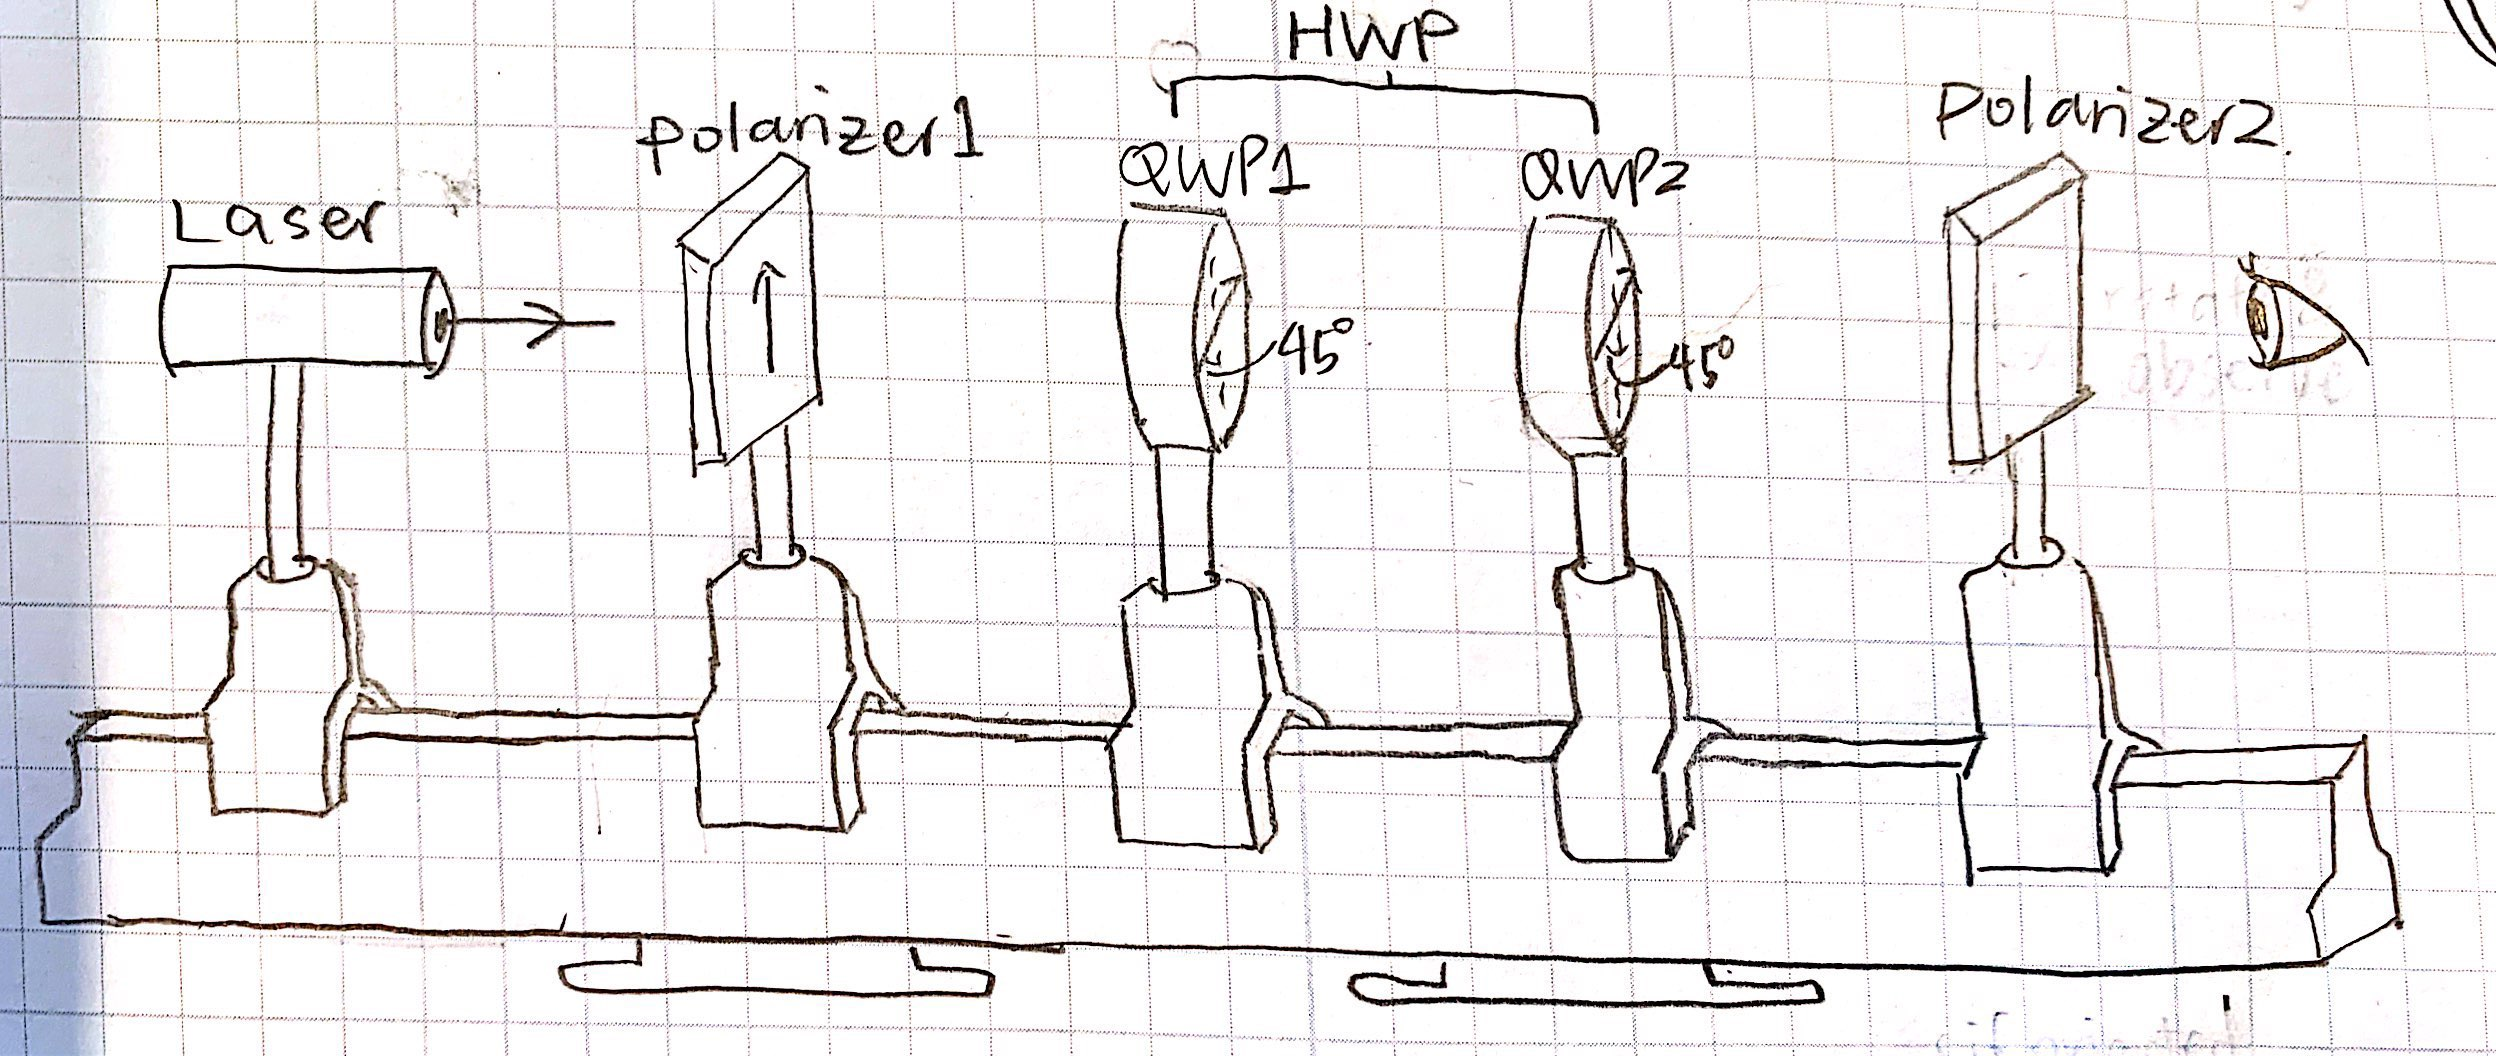
\includegraphics{fig2.jpg}
\caption{Experiment 2}
\end{figure}

\begin{enumerate}
\def\labelenumi{\arabic{enumi}.}
\setcounter{enumi}{1}
\item
  Place a screen where the eye is in the diagram, and place another
  linear polarizer between the second QWP and the screen.
\item
  Rotate the second linear polarizer to determine if the light is at
  least roughly linearly polarized.
\item
  For the second Observation/Analysis, set up materials again according
  to the above diagram, but this time turn the second QWP so its fast
  axis is perpendicular to the first QWP's fast axis. Place a
  photodetector where the eye is in the diagram.
\item
  Take data to demonstrate that when the fast axis of QWP 2 is
  perpendicular to the fast axis of QWP 1, the transmitted light is
  still linearly polarized. Determine the orientation of the
  polarization axis. Compare the measured polarization axis to the
  predicted polarization axis.
\end{enumerate}

\hypertarget{answer}{%
\subsubsection{Answer}\label{answer}}

\hypertarget{observationanalysis-1}{%
\paragraph{Observation/Analysis 1:}\label{observationanalysis-1}}

By turning the second linear polarizer, we observed that the brightness
of the transmitted beam varied sinusoidally as we turned the linear
polarizer. We also observed the transmitted beam was brightest when the
second linear polarizer was horizontal, which indicates the transmitted
beam was horizontally polarized.

This result agreed with theoretical prediction, because a half-wave
plate should decrease the phase of one component of linearly-polarized
light by a factor of \(\frac{\pi}{2}\), and if the half-wave plate is
oriented with fast axis making a \(\frac{\pi}{4}\) with the polarization
angle of the incident light, we expect the transmitted light to be
perpendicularly polarized to the incident light.

\hypertarget{observationanalysis-2}{%
\paragraph{Observation/Analysis 2}\label{observationanalysis-2}}

We predict that the polarization axis will be the same as its original
orientation, because the combination of two QWP will shift both wave
components faster by \(\frac{\pi}{2}\) phase, which has no effect on the
transmission axis of the light.

In the data table below, `theta' denotes the clockwise angle difference
between QWP 2's fast axis and the vertical axis, with unit degree;
`delta\_theta' denotes the error associated with the angle difference,
with unit degree; `I' denotes the intensity of transmitted light, with
unit lux; `delta\_I' denotes the error associated with the intensity,
with unit lux.

    \begin{tcolorbox}[breakable, size=fbox, boxrule=1pt, pad at break*=1mm,colback=cellbackground, colframe=cellborder]
\prompt{In}{incolor}{9}{\hspace{4pt}}
\begin{Verbatim}[commandchars=\\\{\}]
\PY{n}{df}
\end{Verbatim}
\end{tcolorbox}

            \begin{tcolorbox}[breakable, boxrule=.5pt, size=fbox, pad at break*=1mm, opacityfill=0]
\prompt{Out}{outcolor}{9}{\hspace{3.5pt}}
\begin{Verbatim}[commandchars=\\\{\}]
   theta  delta\_theta     I  delta\_I
0      0            1  4270        5
1     15            1  3470        5
2     30            1  2647        5
3     45            1  1392        5
4     60            1   298        5
5     75            1    34        5
6     90            1     6        5
\end{Verbatim}
\end{tcolorbox}
        
    \begin{tcolorbox}[breakable, size=fbox, boxrule=1pt, pad at break*=1mm,colback=cellbackground, colframe=cellborder]
\prompt{In}{incolor}{15}{\hspace{4pt}}
\begin{Verbatim}[commandchars=\\\{\}]
\PY{n}{plt}\PY{o}{.}\PY{n}{errorbar}\PY{p}{(}\PY{n}{df}\PY{o}{.}\PY{n}{theta}\PY{p}{,} \PY{n}{df}\PY{o}{.}\PY{n}{I}\PY{p}{,} \PY{n}{yerr} \PY{o}{=} \PY{n}{df}\PY{o}{.}\PY{n}{delta\PYZus{}I}\PY{p}{)}
\PY{n}{plt}\PY{o}{.}\PY{n}{xlabel}\PY{p}{(}\PY{l+s+s1}{\PYZsq{}}\PY{l+s+s1}{theta(degrees)}\PY{l+s+s1}{\PYZsq{}}\PY{p}{)}
\PY{n}{plt}\PY{o}{.}\PY{n}{ylabel}\PY{p}{(}\PY{l+s+s1}{\PYZsq{}}\PY{l+s+s1}{Intensity(lux)}\PY{l+s+s1}{\PYZsq{}}\PY{p}{)}
\PY{n}{plt}\PY{o}{.}\PY{n}{title}\PY{p}{(}\PY{l+s+s1}{\PYZsq{}}\PY{l+s+s1}{intensity vs. theta}\PY{l+s+s1}{\PYZsq{}}\PY{p}{)}
\PY{n}{plt}\PY{o}{.}\PY{n}{show}\PY{p}{(}\PY{p}{)}
\end{Verbatim}
\end{tcolorbox}

    \begin{center}
    \adjustimage{max size={0.9\linewidth}{0.9\paperheight}}{output_24_0.png}
    \end{center}
    { \hspace*{\fill} \\}
    
    Note: Because the error bars for intensity is very small, they're hardly
visible in the graph above.

    From the data table, we observed that the intensity of transmitted light
varies sinusoidally as the axis of Polarizer 2 rotates, and reaches its
maximum when the axis is vertically oriented. This shows that the light
is still linearly polarized with its polarization axis vertically
oriented, which agrees with our prediction.

    \hypertarget{experiment-3---optical-activity-of-corn-syrup}{%
\section{Experiment 3 - Optical Activity of Corn
Syrup}\label{experiment-3---optical-activity-of-corn-syrup}}

\hypertarget{objective}{%
\subsection{Objective}\label{objective}}

Explore the optical activity of a given sample of corn syrup rotating
the polarization axis of linearly polarized light

\hypertarget{method}{%
\subsection{Method}\label{method}}

Setup as illustrated in the diagram below:

\begin{figure}
\centering
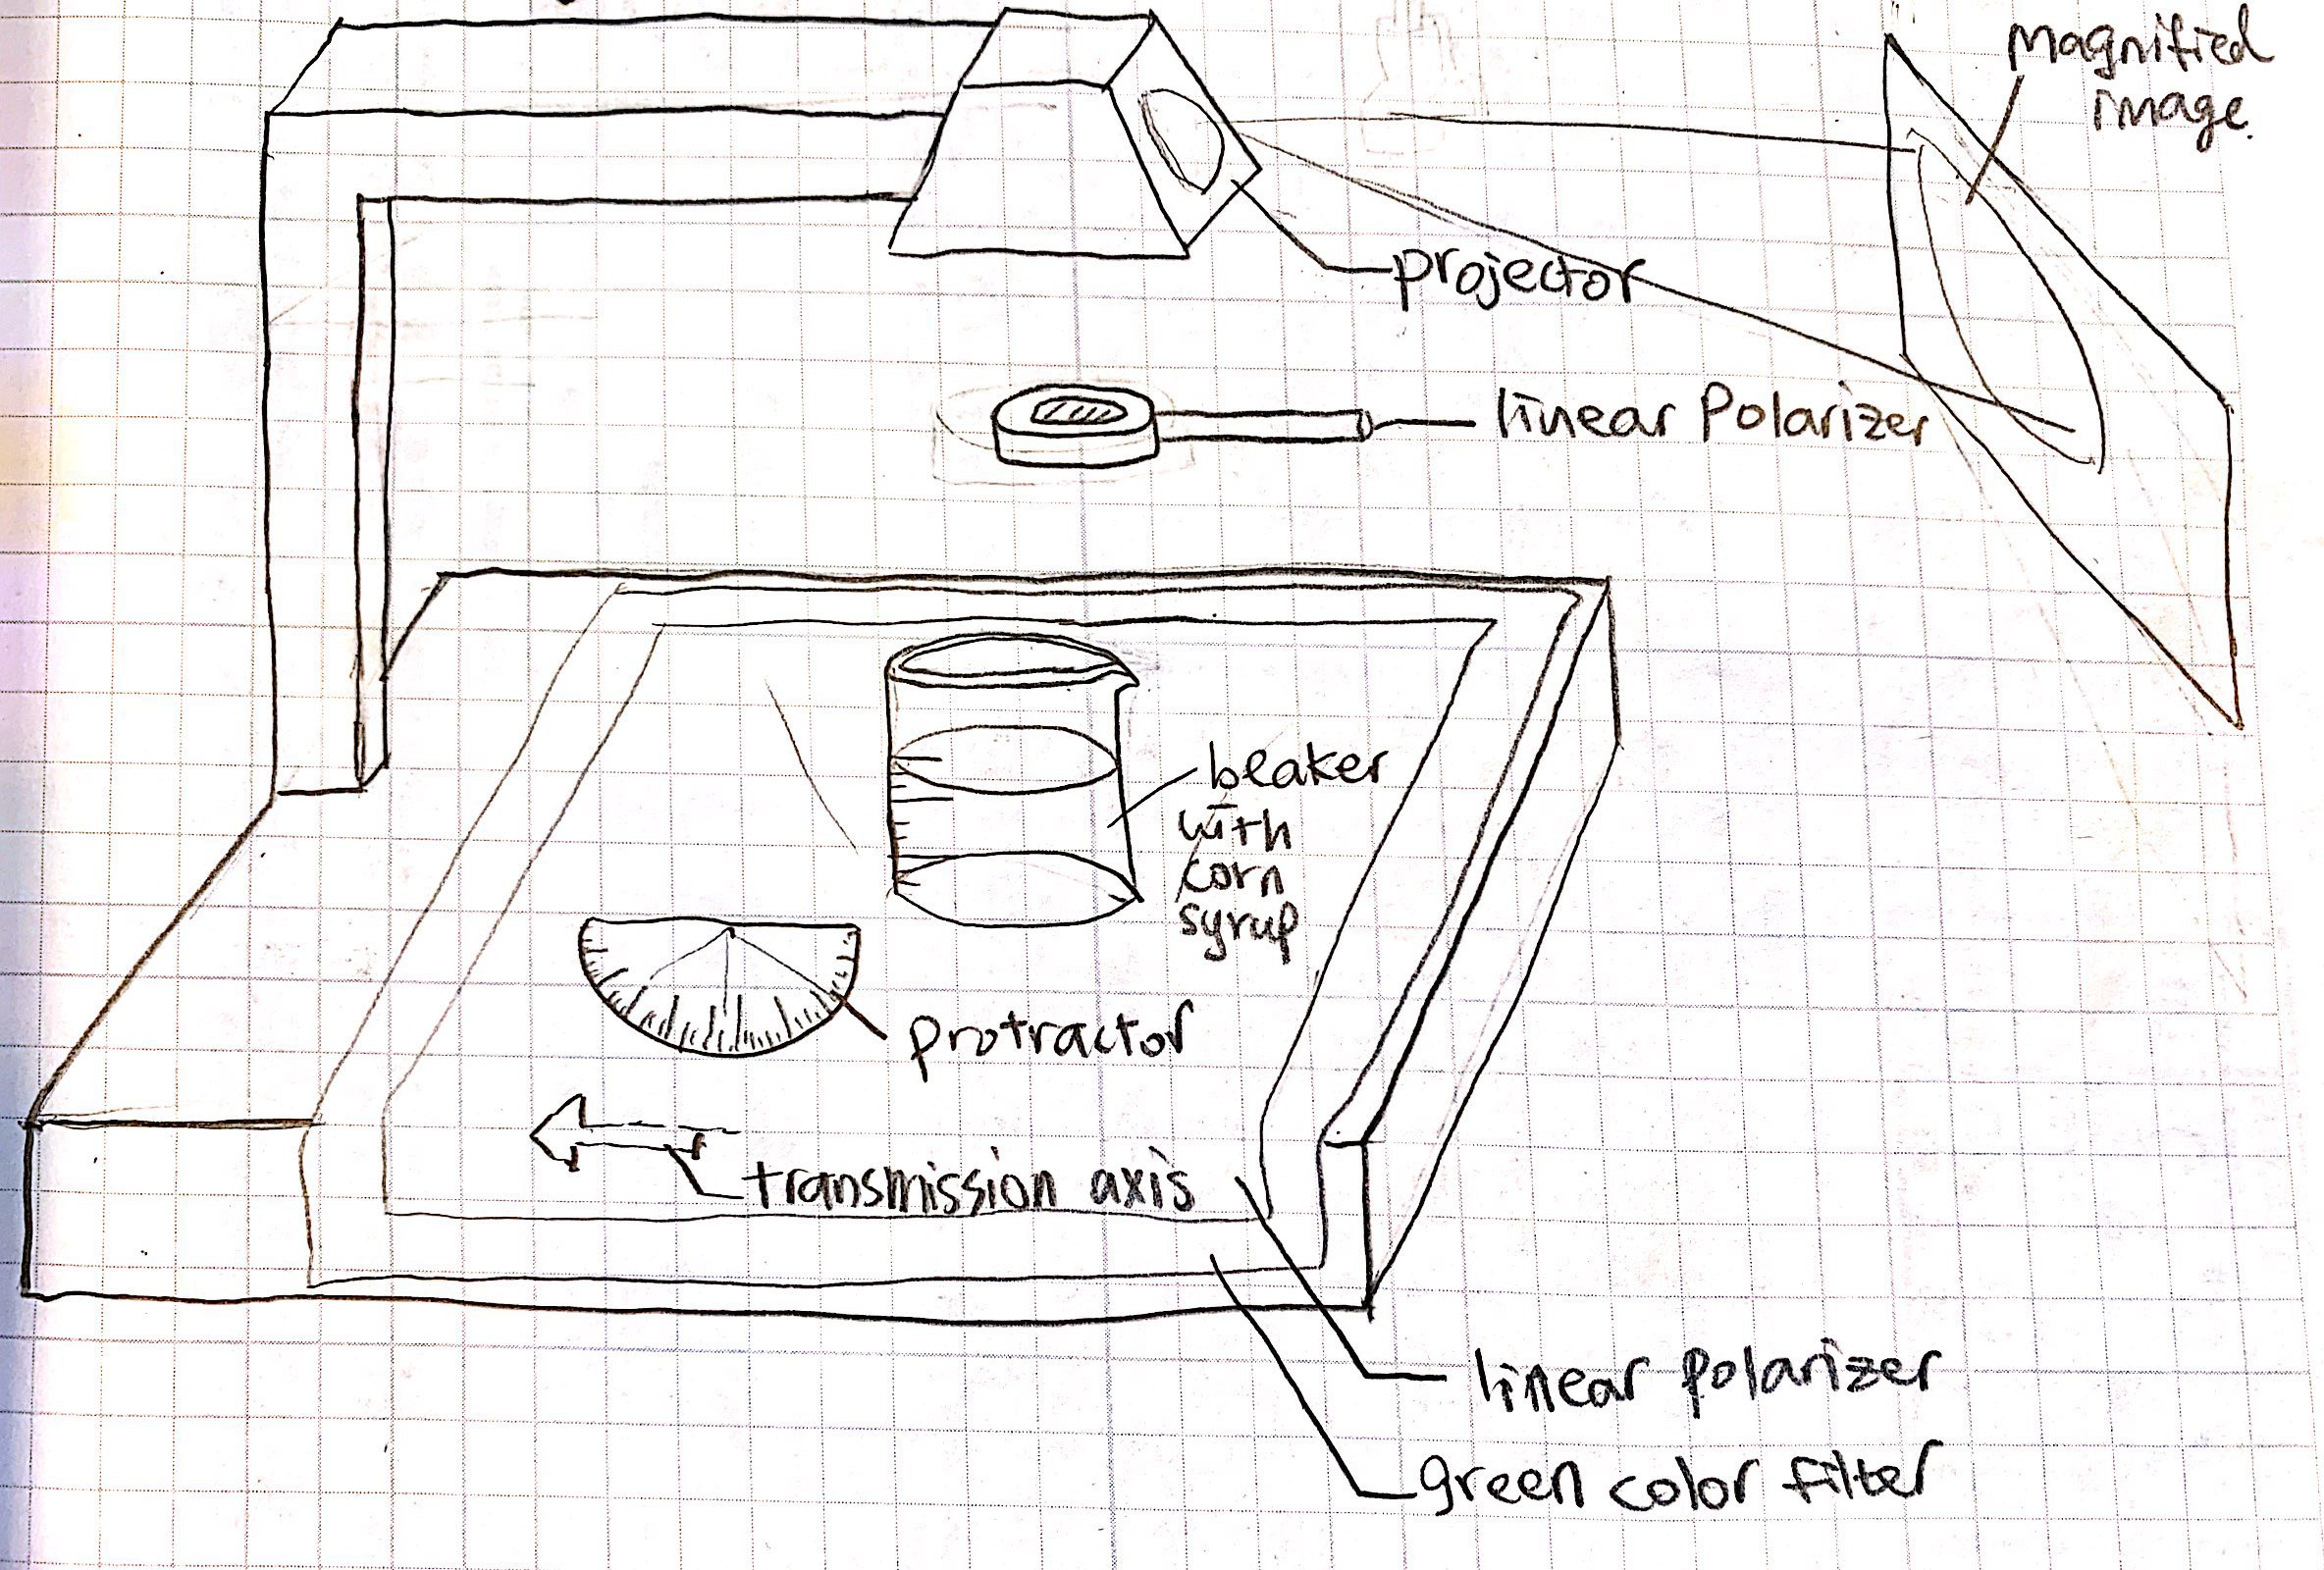
\includegraphics{fig1.jpg}
\caption{Experiment 3}
\end{figure}

Measure the height \(l\) of the corn syrup in each cylinder Determine
the \textbf{optical rotation angle} \(\alpha\) for each corn syrup
sample.

In the data table below, `l' denotes the height of corn syrup, with unit
centimeter; `delta\_l' denotes the error associated with the height,
with unit centimeter; `alpha' denotes the optical rotation angle
clockwise from the positive vertical axis for each corn syrup sample,
with unit degrees; `delta\_alpha' denotes the error associated with the
optical rotation angle, with unit degrees.

    \begin{tcolorbox}[breakable, size=fbox, boxrule=1pt, pad at break*=1mm,colback=cellbackground, colframe=cellborder]
\prompt{In}{incolor}{27}{\hspace{4pt}}
\begin{Verbatim}[commandchars=\\\{\}]
\PY{n}{df1}
\end{Verbatim}
\end{tcolorbox}

            \begin{tcolorbox}[breakable, boxrule=.5pt, size=fbox, pad at break*=1mm, opacityfill=0]
\prompt{Out}{outcolor}{27}{\hspace{3.5pt}}
\begin{Verbatim}[commandchars=\\\{\}]
     l  delta\_l  alpha  delta\_alpha
0  5.1      0.1    -65            1
1  3.4      0.1     74            1
2  2.5      0.1     61            1
3  1.4      0.1     19            1
\end{Verbatim}
\end{tcolorbox}
        
    \hypertarget{data-analysis}{%
\subsection{Data Analysis}\label{data-analysis}}

    \begin{tcolorbox}[breakable, size=fbox, boxrule=1pt, pad at break*=1mm,colback=cellbackground, colframe=cellborder]
\prompt{In}{incolor}{39}{\hspace{4pt}}
\begin{Verbatim}[commandchars=\\\{\}]
\PY{n}{plt}\PY{o}{.}\PY{n}{errorbar}\PY{p}{(}\PY{n}{df1}\PY{o}{.}\PY{n}{l}\PY{p}{,} \PY{n}{df1}\PY{o}{.}\PY{n}{alpha}\PY{p}{,} \PY{n}{yerr} \PY{o}{=} \PY{n}{df1}\PY{o}{.}\PY{n}{delta\PYZus{}alpha}\PY{p}{,} \PY{n}{fmt} \PY{o}{=} \PY{l+s+s1}{\PYZsq{}}\PY{l+s+s1}{.}\PY{l+s+s1}{\PYZsq{}}\PY{p}{)}
\PY{n}{plt}\PY{o}{.}\PY{n}{xlabel}\PY{p}{(}\PY{l+s+s1}{\PYZsq{}}\PY{l+s+s1}{height(cm)}\PY{l+s+s1}{\PYZsq{}}\PY{p}{)}
\PY{n}{plt}\PY{o}{.}\PY{n}{ylabel}\PY{p}{(}\PY{l+s+s1}{\PYZsq{}}\PY{l+s+s1}{alpha(degrees)}\PY{l+s+s1}{\PYZsq{}}\PY{p}{)}
\PY{n}{plt}\PY{o}{.}\PY{n}{title}\PY{p}{(}\PY{l+s+s1}{\PYZsq{}}\PY{l+s+s1}{alpha vs. height}\PY{l+s+s1}{\PYZsq{}}\PY{p}{)}
\PY{n}{plt}\PY{o}{.}\PY{n}{show}\PY{p}{(}\PY{p}{)}
\end{Verbatim}
\end{tcolorbox}

    \begin{center}
    \adjustimage{max size={0.9\linewidth}{0.9\paperheight}}{output_30_0.png}
    \end{center}
    { \hspace*{\fill} \\}
    
    Note: Because the error bars for alpha are very small, they're hardly
visible in the graph above.

b). Using the direct proportionality hypothesis, we yielded that the
gradient of this linear fit model
\(c[\alpha] = 22.22\pm3.45 \text{ }^{\circ}/cm\), with a coefficient of
determination of \(0.975\), which is a fairly good fit.

c). From the given corn syrup concentration, the specific rotation is
\([\alpha] = gradient/c = 66.7\pm10.4^{\circ} mL/cm \cdot g\)

d). Using accepted value of \(52.7^{\circ}mL/cm \cdot g\), the agreement
test value is 0.67. This value is smaller than 1, so our result is in
agreement with the accepted value.

    The following scripts calculated the results in part b)

    \begin{tcolorbox}[breakable, size=fbox, boxrule=1pt, pad at break*=1mm,colback=cellbackground, colframe=cellborder]
\prompt{In}{incolor}{48}{\hspace{4pt}}
\begin{Verbatim}[commandchars=\\\{\}]
\PY{n}{df1}\PY{p}{[}\PY{l+s+s1}{\PYZsq{}}\PY{l+s+s1}{xy}\PY{l+s+s1}{\PYZsq{}}\PY{p}{]} \PY{o}{=} \PY{n}{df1}\PY{p}{[}\PY{l+s+s1}{\PYZsq{}}\PY{l+s+s1}{l}\PY{l+s+s1}{\PYZsq{}}\PY{p}{]} \PY{o}{*} \PY{n}{df1}\PY{p}{[}\PY{l+s+s1}{\PYZsq{}}\PY{l+s+s1}{alpha}\PY{l+s+s1}{\PYZsq{}}\PY{p}{]}
\PY{n}{df1}\PY{p}{[}\PY{l+s+s1}{\PYZsq{}}\PY{l+s+s1}{x\PYZus{}square}\PY{l+s+s1}{\PYZsq{}}\PY{p}{]} \PY{o}{=} \PY{n}{df1}\PY{p}{[}\PY{l+s+s1}{\PYZsq{}}\PY{l+s+s1}{l}\PY{l+s+s1}{\PYZsq{}}\PY{p}{]}\PY{o}{*}\PY{o}{*}\PY{l+m+mi}{2}
\PY{n}{xy\PYZus{}mean} \PY{o}{=} \PY{n}{np}\PY{o}{.}\PY{n}{mean}\PY{p}{(}\PY{n}{df1}\PY{p}{[}\PY{l+s+s1}{\PYZsq{}}\PY{l+s+s1}{xy}\PY{l+s+s1}{\PYZsq{}}\PY{p}{]}\PY{p}{)}
\PY{n}{x\PYZus{}square\PYZus{}mean} \PY{o}{=} \PY{n}{np}\PY{o}{.}\PY{n}{mean}\PY{p}{(}\PY{n}{df1}\PY{p}{[}\PY{l+s+s1}{\PYZsq{}}\PY{l+s+s1}{x\PYZus{}square}\PY{l+s+s1}{\PYZsq{}}\PY{p}{]}\PY{p}{)}
\PY{n}{m\PYZus{}hat} \PY{o}{=} \PY{n}{xy\PYZus{}mean} \PY{o}{/} \PY{n}{x\PYZus{}square\PYZus{}mean}
\PY{n+nb}{print}\PY{p}{(}\PY{n}{m\PYZus{}hat}\PY{p}{)}
\end{Verbatim}
\end{tcolorbox}

    \begin{Verbatim}[commandchars=\\\{\}]
22.219309742245525
\end{Verbatim}

    \begin{tcolorbox}[breakable, size=fbox, boxrule=1pt, pad at break*=1mm,colback=cellbackground, colframe=cellborder]
\prompt{In}{incolor}{54}{\hspace{4pt}}
\begin{Verbatim}[commandchars=\\\{\}]
\PY{n}{df1}\PY{p}{[}\PY{l+s+s1}{\PYZsq{}}\PY{l+s+s1}{y\PYZus{}mhatx}\PY{l+s+s1}{\PYZsq{}}\PY{p}{]} \PY{o}{=} \PY{n}{df1}\PY{p}{[}\PY{l+s+s1}{\PYZsq{}}\PY{l+s+s1}{alpha}\PY{l+s+s1}{\PYZsq{}}\PY{p}{]} \PY{o}{\PYZhy{}} \PY{n}{m\PYZus{}hat} \PY{o}{*} \PY{n}{df1}\PY{p}{[}\PY{l+s+s1}{\PYZsq{}}\PY{l+s+s1}{l}\PY{l+s+s1}{\PYZsq{}}\PY{p}{]}
\PY{n}{df1}\PY{p}{[}\PY{l+s+s1}{\PYZsq{}}\PY{l+s+s1}{ymx\PYZus{}square}\PY{l+s+s1}{\PYZsq{}}\PY{p}{]} \PY{o}{=} \PY{n}{df1}\PY{p}{[}\PY{l+s+s1}{\PYZsq{}}\PY{l+s+s1}{y\PYZus{}mhatx}\PY{l+s+s1}{\PYZsq{}}\PY{p}{]}\PY{o}{*}\PY{o}{*}\PY{l+m+mi}{2}
\PY{n}{ymxsq\PYZus{}sum} \PY{o}{=} \PY{n}{np}\PY{o}{.}\PY{n}{sum}\PY{p}{(}\PY{n}{df1}\PY{p}{[}\PY{l+s+s1}{\PYZsq{}}\PY{l+s+s1}{ymx\PYZus{}square}\PY{l+s+s1}{\PYZsq{}}\PY{p}{]}\PY{p}{)}
\PY{n}{y\PYZus{}error} \PY{o}{=} \PY{n}{np}\PY{o}{.}\PY{n}{sqrt}\PY{p}{(}\PY{l+m+mi}{3} \PY{o}{*} \PY{n}{ymxsq\PYZus{}sum}\PY{p}{)}
\PY{n}{mhat\PYZus{}error} \PY{o}{=} \PY{n}{y\PYZus{}error}\PY{o}{/}\PY{p}{(}\PY{n}{np}\PY{o}{.}\PY{n}{sqrt}\PY{p}{(}\PY{l+m+mi}{4} \PY{o}{*} \PY{n}{x\PYZus{}square\PYZus{}mean}\PY{p}{)}\PY{p}{)}
\PY{n+nb}{print}\PY{p}{(}\PY{n}{mhat\PYZus{}error}\PY{p}{)}
\end{Verbatim}
\end{tcolorbox}

    \begin{Verbatim}[commandchars=\\\{\}]
3.448916959069044
\end{Verbatim}

    \begin{tcolorbox}[breakable, size=fbox, boxrule=1pt, pad at break*=1mm,colback=cellbackground, colframe=cellborder]
\prompt{In}{incolor}{41}{\hspace{4pt}}
\begin{Verbatim}[commandchars=\\\{\}]
\PY{n}{x} \PY{o}{=} \PY{n}{np}\PY{o}{.}\PY{n}{array}\PY{p}{(}\PY{n}{df1}\PY{p}{[}\PY{l+s+s1}{\PYZsq{}}\PY{l+s+s1}{l}\PY{l+s+s1}{\PYZsq{}}\PY{p}{]}\PY{p}{)}\PY{o}{.}\PY{n}{reshape}\PY{p}{(}\PY{o}{\PYZhy{}}\PY{l+m+mi}{1}\PY{p}{,} \PY{l+m+mi}{1}\PY{p}{)}
\PY{n}{y} \PY{o}{=} \PY{n}{df1}\PY{p}{[}\PY{l+s+s1}{\PYZsq{}}\PY{l+s+s1}{alpha}\PY{l+s+s1}{\PYZsq{}}\PY{p}{]}
\PY{n}{model} \PY{o}{=} \PY{n}{LinearRegression}\PY{p}{(}\PY{p}{)}\PY{o}{.}\PY{n}{fit}\PY{p}{(}\PY{n}{x}\PY{p}{,} \PY{n}{y}\PY{p}{)}
\PY{n}{r\PYZus{}sq} \PY{o}{=} \PY{n}{model}\PY{o}{.}\PY{n}{score}\PY{p}{(}\PY{n}{x}\PY{p}{,} \PY{n}{y}\PY{p}{)}
\PY{n+nb}{print}\PY{p}{(}\PY{l+s+s1}{\PYZsq{}}\PY{l+s+s1}{coefficient of determination:}\PY{l+s+s1}{\PYZsq{}}\PY{p}{,} \PY{n}{r\PYZus{}sq}\PY{p}{)}
\PY{n+nb}{print}\PY{p}{(}\PY{l+s+s1}{\PYZsq{}}\PY{l+s+s1}{intercept:}\PY{l+s+s1}{\PYZsq{}}\PY{p}{,} \PY{n}{model}\PY{o}{.}\PY{n}{intercept\PYZus{}}\PY{p}{)}
\PY{n+nb}{print}\PY{p}{(}\PY{l+s+s1}{\PYZsq{}}\PY{l+s+s1}{slope:}\PY{l+s+s1}{\PYZsq{}}\PY{p}{,} \PY{n}{model}\PY{o}{.}\PY{n}{coef\PYZus{}}\PY{p}{)}
\end{Verbatim}
\end{tcolorbox}

    \begin{Verbatim}[commandchars=\\\{\}]
coefficient of determination: 0.9754420008718302
intercept: -10.165531335149865
slope: [24.97275204]
\end{Verbatim}

    The following scripts calculated the results in part c).

    \begin{tcolorbox}[breakable, size=fbox, boxrule=1pt, pad at break*=1mm,colback=cellbackground, colframe=cellborder]
\prompt{In}{incolor}{8}{\hspace{4pt}}
\begin{Verbatim}[commandchars=\\\{\}]
\PY{n}{data} \PY{o}{=} \PY{p}{\PYZob{}}\PY{l+s+s1}{\PYZsq{}}\PY{l+s+s1}{theta}\PY{l+s+s1}{\PYZsq{}}\PY{p}{:} \PY{p}{[}\PY{l+m+mi}{0}\PY{p}{,} \PY{l+m+mi}{15}\PY{p}{,} \PY{l+m+mi}{30}\PY{p}{,} \PY{l+m+mi}{45}\PY{p}{,} \PY{l+m+mi}{60}\PY{p}{,} \PY{l+m+mi}{75}\PY{p}{,} \PY{l+m+mi}{90}\PY{p}{]}\PY{p}{,} 
        \PY{l+s+s1}{\PYZsq{}}\PY{l+s+s1}{delta\PYZus{}theta}\PY{l+s+s1}{\PYZsq{}}\PY{p}{:}\PY{p}{[}\PY{l+m+mi}{1}\PY{p}{,} \PY{l+m+mi}{1}\PY{p}{,} \PY{l+m+mi}{1}\PY{p}{,} \PY{l+m+mi}{1}\PY{p}{,} \PY{l+m+mi}{1}\PY{p}{,} \PY{l+m+mi}{1}\PY{p}{,} \PY{l+m+mi}{1}\PY{p}{]}\PY{p}{,} 
        \PY{l+s+s1}{\PYZsq{}}\PY{l+s+s1}{I}\PY{l+s+s1}{\PYZsq{}}\PY{p}{:} \PY{p}{[}\PY{l+m+mi}{4270}\PY{p}{,} \PY{l+m+mi}{3470}\PY{p}{,} \PY{l+m+mi}{2647}\PY{p}{,} \PY{l+m+mi}{1392}\PY{p}{,} \PY{l+m+mi}{298}\PY{p}{,} \PY{l+m+mi}{34}\PY{p}{,} \PY{l+m+mi}{6}\PY{p}{]}\PY{p}{,} 
        \PY{l+s+s1}{\PYZsq{}}\PY{l+s+s1}{delta\PYZus{}I}\PY{l+s+s1}{\PYZsq{}}\PY{p}{:} \PY{p}{[}\PY{l+m+mi}{5}\PY{p}{,} \PY{l+m+mi}{5}\PY{p}{,} \PY{l+m+mi}{5}\PY{p}{,} \PY{l+m+mi}{5}\PY{p}{,} \PY{l+m+mi}{5}\PY{p}{,} \PY{l+m+mi}{5}\PY{p}{,} \PY{l+m+mi}{5}\PY{p}{]}\PY{p}{\PYZcb{}}
\PY{n}{df} \PY{o}{=} \PY{n}{pd}\PY{o}{.}\PY{n}{DataFrame}\PY{p}{(}\PY{n}{data}\PY{p}{)}
\end{Verbatim}
\end{tcolorbox}

    \begin{tcolorbox}[breakable, size=fbox, boxrule=1pt, pad at break*=1mm,colback=cellbackground, colframe=cellborder]
\prompt{In}{incolor}{38}{\hspace{4pt}}
\begin{Verbatim}[commandchars=\\\{\}]
\PY{n}{data} \PY{o}{=} \PY{p}{\PYZob{}}\PY{l+s+s1}{\PYZsq{}}\PY{l+s+s1}{l}\PY{l+s+s1}{\PYZsq{}}\PY{p}{:} \PY{p}{[}\PY{l+m+mf}{5.1}\PY{p}{,} \PY{l+m+mf}{3.4}\PY{p}{,} \PY{l+m+mf}{2.5}\PY{p}{,} \PY{l+m+mf}{1.4}\PY{p}{]}\PY{p}{,} 
        \PY{l+s+s1}{\PYZsq{}}\PY{l+s+s1}{delta\PYZus{}l}\PY{l+s+s1}{\PYZsq{}}\PY{p}{:} \PY{p}{[}\PY{l+m+mf}{0.1}\PY{p}{,} \PY{l+m+mf}{0.1}\PY{p}{,} \PY{l+m+mf}{0.1}\PY{p}{,} \PY{l+m+mf}{0.1}\PY{p}{]}\PY{p}{,} 
        \PY{l+s+s1}{\PYZsq{}}\PY{l+s+s1}{alpha}\PY{l+s+s1}{\PYZsq{}}\PY{p}{:} \PY{p}{[}\PY{l+m+mi}{115}\PY{p}{,} \PY{l+m+mi}{74}\PY{p}{,} \PY{l+m+mi}{61}\PY{p}{,} \PY{l+m+mi}{19}\PY{p}{]}\PY{p}{,} 
        \PY{l+s+s1}{\PYZsq{}}\PY{l+s+s1}{delta\PYZus{}alpha}\PY{l+s+s1}{\PYZsq{}}\PY{p}{:} \PY{p}{[}\PY{l+m+mi}{1}\PY{p}{,} \PY{l+m+mi}{1}\PY{p}{,} \PY{l+m+mi}{1}\PY{p}{,} \PY{l+m+mi}{1}\PY{p}{]}\PY{p}{\PYZcb{}}
\PY{n}{df1} \PY{o}{=} \PY{n}{pd}\PY{o}{.}\PY{n}{DataFrame}\PY{p}{(}\PY{n}{data}\PY{p}{)}
\end{Verbatim}
\end{tcolorbox}

    \begin{tcolorbox}[breakable, size=fbox, boxrule=1pt, pad at break*=1mm,colback=cellbackground, colframe=cellborder]
\prompt{In}{incolor}{55}{\hspace{4pt}}
\begin{Verbatim}[commandchars=\\\{\}]
\PY{l+m+mf}{22.22}\PY{o}{/}\PY{p}{(}\PY{l+m+mi}{1}\PY{o}{/}\PY{l+m+mi}{3}\PY{p}{)}
\end{Verbatim}
\end{tcolorbox}

            \begin{tcolorbox}[breakable, boxrule=.5pt, size=fbox, pad at break*=1mm, opacityfill=0]
\prompt{Out}{outcolor}{55}{\hspace{3.5pt}}
\begin{Verbatim}[commandchars=\\\{\}]
66.66
\end{Verbatim}
\end{tcolorbox}
        
    \begin{tcolorbox}[breakable, size=fbox, boxrule=1pt, pad at break*=1mm,colback=cellbackground, colframe=cellborder]
\prompt{In}{incolor}{56}{\hspace{4pt}}
\begin{Verbatim}[commandchars=\\\{\}]
\PY{l+m+mf}{3.45}\PY{o}{*}\PY{l+m+mi}{3}
\end{Verbatim}
\end{tcolorbox}

            \begin{tcolorbox}[breakable, boxrule=.5pt, size=fbox, pad at break*=1mm, opacityfill=0]
\prompt{Out}{outcolor}{56}{\hspace{3.5pt}}
\begin{Verbatim}[commandchars=\\\{\}]
10.350000000000001
\end{Verbatim}
\end{tcolorbox}
        
    This is the agreement test in part e)

    \begin{tcolorbox}[breakable, size=fbox, boxrule=1pt, pad at break*=1mm,colback=cellbackground, colframe=cellborder]
\prompt{In}{incolor}{57}{\hspace{4pt}}
\begin{Verbatim}[commandchars=\\\{\}]
\PY{p}{(}\PY{l+m+mf}{66.7} \PY{o}{\PYZhy{}} \PY{l+m+mf}{52.7}\PY{p}{)}\PY{o}{/}\PY{p}{(}\PY{l+m+mi}{2}\PY{o}{*}\PY{l+m+mf}{10.4}\PY{p}{)}
\end{Verbatim}
\end{tcolorbox}

            \begin{tcolorbox}[breakable, boxrule=.5pt, size=fbox, pad at break*=1mm, opacityfill=0]
\prompt{Out}{outcolor}{57}{\hspace{3.5pt}}
\begin{Verbatim}[commandchars=\\\{\}]
0.673076923076923
\end{Verbatim}
\end{tcolorbox}
        
    \hypertarget{experiment-4-brewsters-angle}{%
\subsection{Experiment 4: Brewster's
Angle}\label{experiment-4-brewsters-angle}}

\hypertarget{objective}{%
\paragraph{Objective:}\label{objective}}

\begin{itemize}
\tightlist
\item
  Find Brewster's angle for the glass plate and from this determine the
  index of refraction of the glass.
\end{itemize}

\hypertarget{method-and-experimental-procedure}{%
\paragraph{Method and Experimental
Procedure:}\label{method-and-experimental-procedure}}

Theory:

Fresnel's Equations tell us that at some angle, \(\theta_{Brewster}\),
the reflectance of p-polarized light off a surface goes to zero. If
\(n_1\) is the index of refraction of the environment, and \(n_2\) is
the index of refraction of the material, then Brewster's Angle is given
by:

\[ \theta_{Brewster} = \tan ^{-1}\left(\frac{n_2}{n_1}\right)\]

From this equation we see

\[ n_2  = n_1 \cdot \tan(\theta_B),\]

and therefore,

\[\delta n_2 = n_1 \sec^2(\theta_B)  \cdot\delta \theta_B\]

Equipment:

\begin{itemize}
\tightlist
\item
  Optical Bench
\item
  Bench Stands
\item
  Linear Polarizer
\item
  Laser
\item
  Protractor
\end{itemize}

Procedure:

\begin{enumerate}
\def\labelenumi{\arabic{enumi}.}
\tightlist
\item
  Set up materials as shown below. Be sure that the linear polarizer is
  polarizing the light horizontally so that the light is p-polarized.
\end{enumerate}

\begin{figure}
\centering
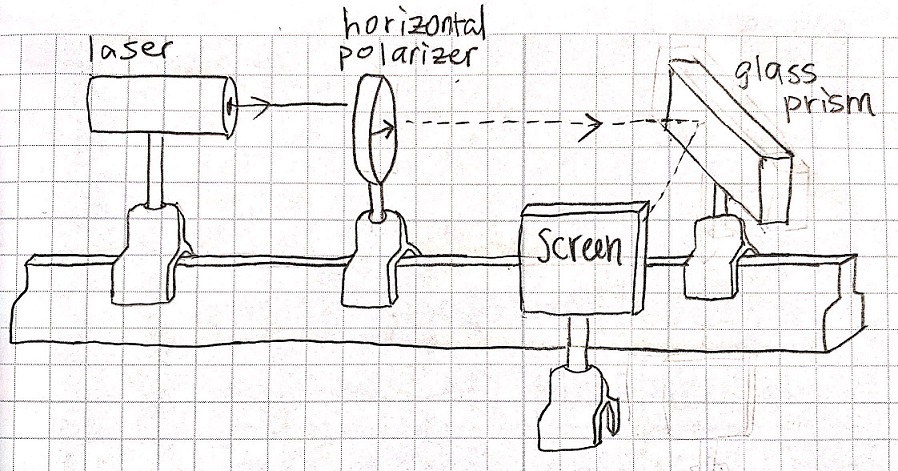
\includegraphics{exp4.jpg}
\caption{Experiment 4}
\end{figure}

\begin{enumerate}
\def\labelenumi{\arabic{enumi}.}
\setcounter{enumi}{1}
\tightlist
\item
  Use the calibration method from Lab 0 to align the laser pointer
  directly down the optical bench.
\item
  Rotate the glass brick until the reflected beam of light disappears.
\item
  Make sure the glass brick is firmly screwed into its bench stand and
  then use a protractor to measure the angle between the incident beam
  and the vector normal to the surface of the glass brick. This is
  Brewster's Angle.
\end{enumerate}

Data Analysis:

We measured
\[\boxed{\theta_{Brewster} = 0.995 \pm 0.017 \text{ Radians}}\]

Using the equation in the theory section and taking \(n_1 = 1\), we
calculate that:

\[\boxed{ n_{glass} = 1.54 \pm 0.06 }\]

Clearly this agrees with the accepted value of \(1.53\). There are two
possible sources of error in this lab. The first is the error associated
with measuring the angle of incidence with the protractor. While this
error did not greatly affect our results, to minimize this error we
could use a more precise protractor. The second source of error dealt
with the fact that near Brewster's Angle, it was very difficult to see
when the light actually disappeared, and therefore difficult to find the
exact angle. Again, this did not greatly affect our results, but if we
wanted more accurate results, then we could have used a photodetector in
a dark room to more precisely determine when the reflected beam of light
disappears.

    \hypertarget{summary-and-conclusions}{%
\subsection{Summary and Conclusions:}\label{summary-and-conclusions}}

In this lab, we were experimenting with the different types of polarized
Light. The purpose of the lab was to learn to identify unpolarized,
linearly polarized, and circularly polarized light, explore Malus's Law
and Brewster's Angle, and study optical activity. In experiment one, we
verified Malus's Law. In Experiment 2, we learned about circular
polarization and how to determine the polarization of any light source.
In Experiment 3, we learned how to find the specific rotation of a
liquid, and finally in Experiment 4, we found Brewster's angle for Crown
Glass. Thus we completed our objectives for this lab through a variety
of different experiments.

    \hypertarget{contributions-of-each-member}{%
\subsection{Contributions of Each
Member}\label{contributions-of-each-member}}

We both did 50\% of the total work on this lab, both on the actual lab
work and writing the lab report.

    \hypertarget{references}{%
\subsection{References}\label{references}}

We used python in this lab, and the open source python Libraries,
Pandas, Matplotlib, and NumPy.

The following scripts were used in experiment 1 to create the data
tables.

    \begin{tcolorbox}[breakable, size=fbox, boxrule=1pt, pad at break*=1mm,colback=cellbackground, colframe=cellborder]
\prompt{In}{incolor}{78}{\hspace{4pt}}
\begin{Verbatim}[commandchars=\\\{\}]
\PY{k+kn}{import} \PY{n+nn}{pandas} \PY{k}{as} \PY{n+nn}{pd}
\PY{k+kn}{from} \PY{n+nn}{math} \PY{k}{import} \PY{o}{*}
\PY{k+kn}{import} \PY{n+nn}{matplotlib}\PY{n+nn}{.}\PY{n+nn}{pyplot} \PY{k}{as} \PY{n+nn}{plt}
\PY{k+kn}{from} \PY{n+nn}{IPython}\PY{n+nn}{.}\PY{n+nn}{display} \PY{k}{import} \PY{n}{Image}
\PY{n}{im1} \PY{o}{=} \PY{n}{Image}\PY{p}{(}\PY{l+s+s1}{\PYZsq{}}\PY{l+s+s1}{exp4.jpg}\PY{l+s+s1}{\PYZsq{}}\PY{p}{)}
\end{Verbatim}
\end{tcolorbox}

    \begin{tcolorbox}[breakable, size=fbox, boxrule=1pt, pad at break*=1mm,colback=cellbackground, colframe=cellborder]
\prompt{In}{incolor}{9}{\hspace{4pt}}
\begin{Verbatim}[commandchars=\\\{\}]
\PY{n}{data1\PYZus{}dict} \PY{o}{=} \PY{p}{\PYZob{}}\PY{l+s+s1}{\PYZsq{}}\PY{l+s+s1}{theta}\PY{l+s+s1}{\PYZsq{}}\PY{p}{:} \PY{p}{[}\PY{l+m+mi}{0}\PY{p}{,} \PY{l+m+mi}{10}\PY{p}{,} \PY{l+m+mi}{20}\PY{p}{,} \PY{l+m+mi}{30}\PY{p}{,} \PY{l+m+mi}{40}\PY{p}{,} \PY{l+m+mi}{50}\PY{p}{,} \PY{l+m+mi}{60}\PY{p}{,} \PY{l+m+mi}{70}\PY{p}{,} \PY{l+m+mi}{80}\PY{p}{,} \PY{l+m+mi}{90}\PY{p}{]}\PY{p}{,}
              \PY{l+s+s1}{\PYZsq{}}\PY{l+s+s1}{delta\PYZus{}theta}\PY{l+s+s1}{\PYZsq{}}\PY{p}{:} \PY{p}{[}\PY{l+m+mi}{2}\PY{p}{,} \PY{l+m+mi}{2}\PY{p}{,} \PY{l+m+mi}{2}\PY{p}{,} \PY{l+m+mi}{2}\PY{p}{,} \PY{l+m+mi}{2}\PY{p}{,} \PY{l+m+mi}{2}\PY{p}{,} \PY{l+m+mi}{2}\PY{p}{,} \PY{l+m+mi}{2}\PY{p}{,} \PY{l+m+mi}{2}\PY{p}{,} \PY{l+m+mi}{2}\PY{p}{]}\PY{p}{,}
             \PY{l+s+s1}{\PYZsq{}}\PY{l+s+s1}{I}\PY{l+s+s1}{\PYZsq{}}\PY{p}{:} \PY{p}{[}\PY{l+m+mi}{6842}\PY{p}{,} \PY{l+m+mi}{6430}\PY{p}{,} \PY{l+m+mi}{6060}\PY{p}{,} \PY{l+m+mi}{5130}\PY{p}{,} \PY{l+m+mi}{4155}\PY{p}{,} \PY{l+m+mi}{3060}\PY{p}{,} \PY{l+m+mi}{1868}\PY{p}{,} \PY{l+m+mi}{1029}\PY{p}{,} \PY{l+m+mi}{350}\PY{p}{,} \PY{l+m+mi}{54}\PY{p}{]}\PY{p}{,}
             \PY{l+s+s1}{\PYZsq{}}\PY{l+s+s1}{delta\PYZus{}I}\PY{l+s+s1}{\PYZsq{}} \PY{p}{:} \PY{p}{[}\PY{l+m+mi}{30}\PY{p}{,} \PY{l+m+mi}{30}\PY{p}{,} \PY{l+m+mi}{30}\PY{p}{,} \PY{l+m+mi}{30}\PY{p}{,} \PY{l+m+mi}{30}\PY{p}{,} \PY{l+m+mi}{20}\PY{p}{,} \PY{l+m+mi}{20}\PY{p}{,} \PY{l+m+mi}{10}\PY{p}{,} \PY{l+m+mi}{10}\PY{p}{,} \PY{l+m+mi}{5}\PY{p}{]}\PY{p}{\PYZcb{}}
\PY{n}{data1} \PY{o}{=} \PY{n}{pd}\PY{o}{.}\PY{n}{DataFrame}\PY{p}{(}\PY{n}{data1\PYZus{}dict}\PY{p}{)}
\end{Verbatim}
\end{tcolorbox}

    \begin{tcolorbox}[breakable, size=fbox, boxrule=1pt, pad at break*=1mm,colback=cellbackground, colframe=cellborder]
\prompt{In}{incolor}{17}{\hspace{4pt}}
\begin{Verbatim}[commandchars=\\\{\}]
\PY{n}{x} \PY{o}{=} \PY{p}{[}\PY{p}{]}
\PY{n}{dx} \PY{o}{=} \PY{p}{[}\PY{p}{]}
\PY{k}{for} \PY{n}{index}\PY{p}{,} \PY{n}{row} \PY{o+ow}{in} \PY{n}{data1}\PY{o}{.}\PY{n}{iterrows}\PY{p}{(}\PY{p}{)}\PY{p}{:}
    \PY{n}{x}\PY{o}{.}\PY{n}{append}\PY{p}{(}\PY{n}{cos}\PY{p}{(}\PY{n}{row}\PY{o}{.}\PY{n}{theta} \PY{o}{*} \PY{n}{pi} \PY{o}{/} \PY{l+m+mi}{180}\PY{p}{)}\PY{o}{*}\PY{o}{*}\PY{l+m+mi}{2}\PY{p}{)}
    \PY{n}{dx}\PY{o}{.}\PY{n}{append}\PY{p}{(}\PY{n}{sin}\PY{p}{(}\PY{n}{row}\PY{o}{.}\PY{n}{delta\PYZus{}theta} \PY{o}{*} \PY{n}{pi} \PY{o}{/} \PY{l+m+mi}{90}\PY{p}{)} \PY{o}{*} \PY{n}{row}\PY{o}{.}\PY{n}{delta\PYZus{}theta}\PY{p}{)}
\PY{n}{datax} \PY{o}{=} \PY{n}{pd}\PY{o}{.}\PY{n}{DataFrame}\PY{p}{(}\PY{p}{)}
\PY{n}{datax}\PY{p}{[}\PY{l+s+s1}{\PYZsq{}}\PY{l+s+s1}{x}\PY{l+s+s1}{\PYZsq{}}\PY{p}{]} \PY{o}{=} \PY{n}{x}
\PY{n}{datax}\PY{p}{[}\PY{l+s+s1}{\PYZsq{}}\PY{l+s+s1}{delta\PYZus{}x}\PY{l+s+s1}{\PYZsq{}}\PY{p}{]} \PY{o}{=} \PY{n}{dx}
\PY{n}{datax}\PY{p}{[}\PY{l+s+s1}{\PYZsq{}}\PY{l+s+s1}{I}\PY{l+s+s1}{\PYZsq{}}\PY{p}{]} \PY{o}{=} \PY{n}{data1}\PY{o}{.}\PY{n}{I}
\PY{n}{datax}\PY{p}{[}\PY{l+s+s1}{\PYZsq{}}\PY{l+s+s1}{delta\PYZus{}I}\PY{l+s+s1}{\PYZsq{}}\PY{p}{]} \PY{o}{=} \PY{n}{data1}\PY{o}{.}\PY{n}{delta\PYZus{}I}
\end{Verbatim}
\end{tcolorbox}


    % Add a bibliography block to the postdoc
    
    
    
    \end{document}
